\documentclass[12pt, a4paper, twoside, openright]{book}

\usepackage[french]{babel}
\usepackage[T1]{fontenc}
\usepackage[utf8]{inputenc}
\usepackage{lmodern}
\usepackage{graphicx}
\usepackage{hyperref}
\usepackage{listings}
\usepackage{graphicx}
\usepackage{microtype}
\usepackage{glossaries}
\usepackage{color}
\usepackage{here}
\usepackage{float}

\makeglossaries %à la suite de la déclaration de package
\newglossaryentry{table}
        {name={table},
        plural={tables},
        description={Ensemble d'\textit{attributs}.
        dans une base de données relationnelle, chaque ligne d'une table (nommée \textit{tuple}) est identifiée
        par un attribut ou groupe d'attributs
        uniques dans la table, que l'on nomme \textit{clée primaire}.
        Pour simplifier, on peut voir les tables comme des tableaux à une entrée : le nombre de colonnes est fixé, en revanche le nombre de lignes ne l'est pas. La figure \ref{exemple_table} représente une table}}

\newglossaryentry{tuple}
        {name={tuple},
        plural={tuples},
        description={Une \textit{ligne} de données dans une table. Une table contient de 0 à n tuples}}
        
        
\newglossaryentry{JDBC}
{
  name=JDBC,
  description={Java DataBase Connectivity est une interface de programmation permettant de manipuler des bases de données avec des objets. Les systèmes de gestion de base de données doivent fournir un pilote JDBC correspondant à l'implémentation de cette interface}
}

\newglossaryentry{JRE}
{
  name=JRE,
  description={Java Runtime Environment correspond à l'environnement d'exécution d'une application Java. Cet environnement est composé d'une machine virtuelle chargée d'exécuter les fichiers compilées ainsi que des bibliothèques standards fournies par Java}
}

\newglossaryentry{MVC}
{
  name=MVC,
  description={Modèle-Vue-Contrôleur est une façon d'organiser le code de programmation qui est optimale pour les logiciels ayant une interface graphique}
}

\newglossaryentry{commit}
{
  name=commit,
  description={Instruction demandant au SGBD de valider sur la base de données toutes les actions préalablement mises en "cache". Les modifications effectuées deviennent visibles pour les autres utilisateurs du SGBD}
}

\newglossaryentry{attribut}
        {name={attribut},
        plural={attributs},
        description={Un nom de colonne dans une table, également appelé \textit{champ}.
        Une table contient au moins un attribut}}
        
\newglossaryentry{data}{
        name={donnée},
        plural={données},
        description={Valeur brute, sans signification si aucun contexte n'est disponible. Du croisement des données résulte de l'information}}

\newglossaryentry{bdd}{
        name={base de données},
        plural={bases de données},
        description={Abrégé \textit{BD}. Outil permettant de stocker et de retrouver des ensembles des données.
        Dans ce rapport, ne sont mentionnées que des bases de données informatisées et relationelles}}

\newglossaryentry{bddr}{
        name={base de données relationnelle},
        plural={bases de données relationnelles},
        description={Abrégé \textit{BDR}. Il existe plusieurs types de bases de données.
        Dans ce rapport, ne sont mentionnées que des bases de données \textit{relationnelles}.
        Les données sont stockées dans des \textit{tables}, et les tables sont reliées entre elles par leurs clées primaires}}
        
        
\newacronym[plural={LDD},
        first={Langage de Définition des Données (LDD)},
        firstplural={Langages de Définition des Données}]
        {ldd}
        {LDD}
        {Langage de Définition des Données, un sous-ensemble du langage SQL permettant de décrire la structure des tables et les relations entre elles. Très grossièrement, le LDD permet de définir les tables et leurs colonnes}

\newacronym[plural={LMD},
        first={Langage de Manipulation des Données (LMD)},
        firstplural={Langages de Manipulation des données}]
        {lmd}
        {LMD}
        {Langage de Manipulation des Données, un sous-ensemble du SQL permettant d'effectuer les opérations CRUD sur les données contenues dans les tables}

\newacronym[plural={SQL},
        first={Structured Query Language (SQL)}]
        {sql}
        {SQL}
        {Structured Query Langage, un langage déclaratif et normé permettant d'utiliser les bases de données relationelles, largement inspiré par Codd en 1970 et devenu un standart aux Etats-Unis en 1984}

\newacronym[first={Create, Read, Update, Delete (CRUD)}]
                           {crud}
                           {CRUD}
                           {Create, Read, Update, Delete sont les quatre opérations basiques à effectuer sur des enregistrements de données, respectivement : en ajouter des nouveaux, les lire, les mettre à jour et les effacer}

\newacronym[first={système d'Information (SI)},
                           firstplural={Systèmes d'Information (SI)}]
                           {si}
                           {SI}
                           {Le Système d'Information est un ensemble organisé de ressources qui permet de collecter, stocker, traiter et distribuer de l'information}

\newacronym[first={Système de Gestion de Base de Données (SGBD)},
                           firstplural={Systèmes de Gestion de Base de Données (SGBD)},
                           plural={SGBD}]
                           {sgbd}
                           {SGBD}
                           {Système de Gestion de Base de Données, logiciel permettant la définition et la manipulation des bases de données. Dans ce rapport, ne sont mentionnés que des logiciels agissant sur des bases de données relationnelles}

\newglossaryentry{query}
        {name={requête SQL},
        plural={requêtes SQL},
        description={Une requête SQL est le nom couramment associé à du code SQL fonctionnel qui interroge ou agit sur la base de données}}

\newacronym[first={Interface Homme-Machine (IHM)},
	firstplural={Interfaces Homme-Machine (IHM)},
        plural={IHM}]
	{ihm}
	{IHM}
	{Interface Homme-Machine, l'ensemble des moyens mis en oeuvre par l'homme pour communiquer avec la machine.
	Dans ce rapport, les IHM désignent les \textit{fenêtres} développées pour l'application}

\newglossaryentry{constraint}
        {name={contrainte},
        plural={contraintes},
        description={Restriction sur la saisie des données. Elles sont définies en SQL}}

\newglossaryentry{primarykey}
        {name={clée primaire},
        plural={clées primaires},
        description={Contrainte désignant un ou plusieurs attributs comme étant identifiants de la table et non nuls. La valeur d'une clée primaire est différente sur chaque tuple d'une table}}

\newacronym[first={Query By Example (QBE)},
        firstplural={Queries By Example (QBE)}]
        {qbe}
        {QBE}
        {Query By Example, IHM permettant de réaliser des requêtes SQL compliquées au moyens de clics de souris, de drag-and-drop et autres
        facilités ne demandant pas de connaître le langage SQL}

\newacronym[first={Integrated Development Environment (IDE)},
                              plural={IDE}]
        {IDE}
        {IDE}
        {Integrated Development Environment, ensemble d'outils nécessaire à la programmation, regroupés en un logiciel (compilateur, éditeur de liens, débogeur, auto-complétion etc)}
		

\newacronym[first={Object Relational Mapping (ORM)}]
        {orm}
        {ORM}
        {Object Relational Mapping, technique visant à convertir des groupes de données vers des instances, pour les manipuler avec un langage objet}

\newglossaryentry{mock}
		{
		name={mock},
		plural={mocks},
		description={Objet simulé qui reproduit le comportement d'un objet réel mais de façon contrôlée, c'est-à-dire que l'on connait par avance les résultats que vont retourner les méthodes appelées sur cet objet. C'est utile pour tester individuellement des classes qui sont dépendantes d'un système externe non accessible dans un contexte de test (que ce soit de façon fonctionnelle ou par soucis de rapidité)}
		}

\newacronym[first={Développement Piloté par les Tests (TDD)},
	firstplural={Développements Pilotés par les Tests}]
	{tdd}
	{TDD}
	{Le Développement Piloté par les Tests(\textit{test-driven development}), 
	est une technique de développement de logiciels qui préconise d'écrire les \textbf{tests unitaires} avant d'écrire le \textbf{code source} d'un logiciel}

\newacronym[first={Data Access Object (DAO)},
                        firstplural={Data Access Objects}]
        {dao}
        {DAO}
        {Data Access Object, couche de l'application permettant d'enregistrer les données sur un système de stockage, comme par exemple une base de données}


%define
\newcommand{\fontconsolas}[1]{\fontfamily{pag}\selectfont 
#1
}

\newcommand{\exemple}[1]{\newline\newline
\begin{center}
\parbox{10cm}{\textcolor[rgb]{0.5,0.5,0.5}{\fontconsolas{#1}}}
\end{center}
}

\newcommand{\sgbd}{\textbf{Système de Gestion de Base de Données}}
%end define

\title{Interface homme-machine pour gestion de bases de données.}
\author{ALCANTUD Gaël \\ BULATOVIC Alexandre \\ MAURY Adrian \\ UGOLINI Romain \\ \\tuteur : PALLEJA Xavier}
\date{20/02/2017}


\begin{document}
\frontmatter
\maketitle

\thispagestyle{empty}
\chapter*{Remerciements}



Premièrement nous tenons à remercier notre tuteur de projet, \textbf{M. Xavier PALLEJA}, pour avoir encadré ce projet et nous avoir guidé dans la réalisation de l'application à l'aide d'un cycle de développement itératif.

Nous apprécions grandement sa forte implication dans le projet et nous tenons à lui en faire part.

\bigbreak

Nous remercions également les différentes personnes travaillant à l'IUT nous ayant permis d'avancer le projet en mettant à disposition des salles informatiques, notamment les techniciens réseau.

\bigbreak
Enfin, nous remercions \textbf{M. Francis GARCIA} pour son rôle de chef de département informatique et d'avoir fait en sorte que tout se passe au mieux.

De même nous remercions notre professeur de communication \textbf{M. Alain RAIBAUT} pour ses cours qui nous ont été utile à la rédaction de ce rapport ainsi que les précieux conseils donnés sur la façon de gérer une présentation orale.


\tableofcontents
\listoffigures
\printglossaries

\mainmatter
\chapter{Introduction}
Les \glspl{bdd} sont des outils permettant de stocker et retrouver des \glspl{data}. 
Elles se trouvent au coeur des \glspl{si}, et sont indispensables aux entreprises.
En informatique, elles sont numérisées, définies et manipulées grâce à des logiciels nommés \glspl{sgbd}.

Il existe différents types de bases de données, mais le marché reste dominé par les \glspl{bddr}\footnote{\label{part_de_marché_relationnel}
Classement des \glspl{sgbd} les plus populaires : \url{http://db-engines.com/en/ranking}}.
Ces dernières sont gérées par des SGBD relationnels (dit SGBDR) 
dont les plus connus sont Oracle, MySQL et PostgreSQL.

Ces logiciels permettent de définir et de manipuler des bases de données par le biais du \gls{sql}, 
langage déclaratif et normé qui reste le premier et le plus exhaustif des moyens de gérer une base de données relationnelle .

Le \gls{sql} est un frein pour les utilisateurs : s'ils ne connaissent pas le langage, ils ne peuvent pas utiliser de base de données.
Certaines applications, comme \textit{Access}, \textit{LOBase} ou encore \textit{phpMyAdmin} proposent une alternative au SQL grâce à des 
\glspl{ihm}: il est possible de définir les données ou de les manipuler par des clics de boutons, des glisser-déplacer, des cases à cocher ou encore de la saisie
de texte non codé. 

Le but de ce projet tuteuré est de réaliser une application permettant d'utiliser certaines fonctionnalités des
\gls{sgbd} \underline{sans} 
utilser de \gls{sql}, et ce sur n'importe quel \gls{sgbd}.
\footnote{\label{sgbd_et_sgbdr}Dans ce rapport, le terme \gls{sgbd} signifie SGBDR.}
Pour cela, il propose une série d'IHM qui en reprennent certaines fonctionnalités,
à savoir le \gls{ldd} et le \gls{lmd}.

Les utilisateurs finaux de l'application sont les élèves de première année du DUT Informatique, pour
les aider à découvrir les bases de données.

Ce document présente les différentes phases de création de cette application : l'analyse, la conception, le développement et les tests.
Un manuel d'utilisation est disponible dans les dernières pages.

Afin de mieux situer l'application, la figure \ref{sans_idb_schema} montre l'utilisation classique d'un SGBD et 
la figure \ref{avec_idb_schema} l'utilisation de l'application développée.

\begin{figure}[!h]
  \centering
  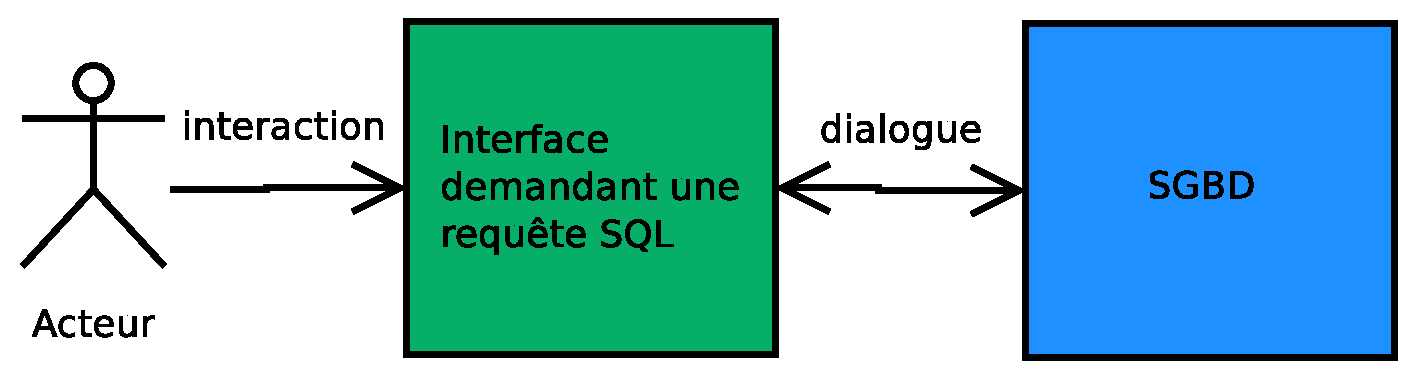
\includegraphics[width=14cm]{images/sans_idb.eps}
  \caption{Utilisation classique d'un SGBD.}
  \label{sans_idb_schema}
\end{figure}

\begin{figure}[!h]
  \centering
  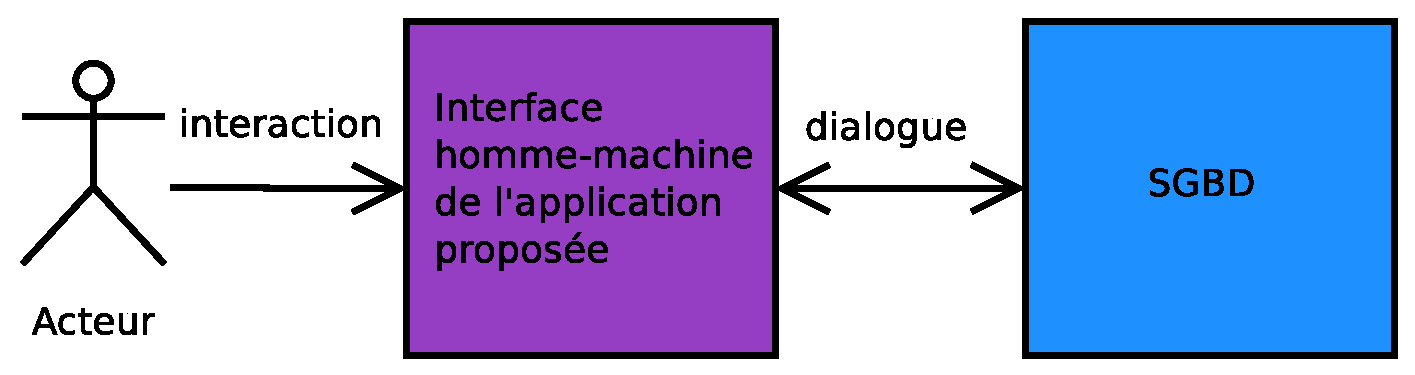
\includegraphics[width=14cm]{images/avec_idb.eps}
  \caption{Utilisation d'un SGBD avec l'application du projet.}
  \label{avec_idb_schema}
\end{figure}

\begin{figure}[!h]
  \centering
  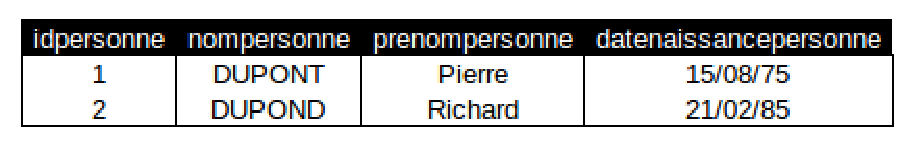
\includegraphics[width=14cm]{images/exemple_table.eps}
  \caption{Un exemple de table avec deux tuples et quatre attributs.}
  \label{exemple_table}
\end{figure}


\chapter{Analyse}
Comme mentionné précédemment, les SGBDR sont les plus utilisés des SGBD. Ils permettent de manipuler des bases de données relationnelles
par le biais du langage SQL. Puisque ce langage nécessite un certain apprentissage, un utilisateur ne le connaissant pas ne peut pas se servir
d'une base de données.

Ce projet tuteuré demande le développement d'une application permettant d'utiliser une base de données suivant deux directives :
\begin{itemize}
\item pas besoin d'utiliser le SQL,
\item compatible avec n'importe quel SGBD.
\end{itemize}

\section{Les fonctionnalités d'un SGBD}
L'application propose des fonctionnalités vues durant le cursus à l'IUT.

\subsection{Le \gls{ldd}}
Le langage de définition des données permet de structurer une base de données.
Il ne s'intêresse pas aux données contenues dans les tables
\footnote{\label{interet_ldd}Le LDD prend en compte les données contenues dans les tables et peut agir dessus, mais c'est une conséquence, pas son rôle.}, mais aux tables elles même. Le LDD est séparé en trois instructions:

\subsubsection{CREATE TABLE}
Permet de créer une \gls{table}. Dans un SGBD, les tables sont nommées, chaque nom est unique.
Une table est créée avec au moins un attribut dont il faut préciser le type de données (texte, nombre, date etc.) et la taille.
Des \glspl{constraint} supplémentaires peuvent être ajoutées, comme par exemple les \glspl{primarykey} \footnote{\label{contrainte_clée_primaire}Voir glossaire.}ou encore des \textit{NOT NULL}.

La \gls{query} suivante montre la création d'une table nommée PERSONNES, qui contient les attributs \textit{idpersonne}, \textit{nompersonne}, \textit{taillepersonne} et \textit{datenaissancepersonne}.

  \begin{lstlisting}
    CREATE TABLE PERSONNES
    (
    idpersonne CHAR(5),
    nompersonne VARCHAR(30),
    taillepersonne NUMBER,
    datenaissancepersonne DATE
    );
  \end{lstlisting}


\subsubsection{ALTER TABLE}
Permet de revenir sur ce qui a été fait avec CREATE TABLE.
L'instruction permet d'ajouter, supprimer ou modifier des \glspl{attribut}, des contraintes, des index...

Cette instruction se comporte différemment selon qu'une table soit vide ou remplie de lignes de données (\glspl{tuple}).
Par exemple, ajouter une contrainte NOT NULL sur une colonne possédant déjà des tuples nuls n'est pas possible. Ce problème n'existe pas sur une table vide.

La requête SQL suivante modifie la table \textit{PERSONNES} pour y ajouter une contrainte de clée primaire nommée \textit{pk\_personnes} sur l'attribut \textit{idpersonne}.

\begin{lstlisting}
  ALTER TABLE PERSONNES
  (
  ADD CONSTRAINT pk_personnes PRIMARY KEY (idpersonne)
  );
\end{lstlisting}

\subsubsection{DROP TABLE}
Permet de supprimer une table et les données qu'elle contient.
Dans une base de données relationnelles, les tables sont liées entre elles par des attributs.
La supression d'une table peut entraîner la supression de données dans d'autres tables, en fonction du schéma relationnel de la base.

La requête SQL suivante supprime la table \textit{PERSONNES} de la base de données.
\begin{lstlisting}
  DROP TABLE PERSONNES;
\end{lstlisting}

\subsection{Le \gls{lmd}}
Le langage de manipulation des données permet d'affectuer des actions de \gls{crud} sur ce que contiennent les tables.
En d'autres termes, il agit sur les tuples.

\subsubsection{Create}
Il d'agit de créer un nouveau tuple dans une table.
La requête SQL suivante permet d'ajouter un tuple de clée primaire \textit{00001} dans la table \textit{PERSONNES}.
\begin{lstlisting}
  INSERT INTO PERSONNES
  (idpersonne, nompersonne, taillepersonne,
  datenaissancepersonne)
  VALUES
  ('00001', 'DUPONT', 'Jean', '06/08/1985');
\end{lstlisting}

\subsubsection{Read}
Il s'agit de récupérer, lire, croiser des données que contiennent les tables.
Les requêtes SQL  "read" peuvent être très complexes.
Certains SGBD proposent des \glspl{qbe}
\footnote{Access, LOBase, phpMyAdmin...}pour créer ces requêtes sans manipuler de SQL.
Celle qui est écrite juste après est simple et permet de retrouver le nom de la \textit{PERSONNES} numéro "00001".
\begin{lstlisting}
  SELECT PERSONNES.nompersonne
  FROM PERSONNES
  WHERE PERSONNES.idpersonne = '00001';
\end{lstlisting}

\subsubsection{Update}
Il s'agit de modifier un ou plusieurs tuples qui existent déjà dans la base de données.
La requête SQL suivante remplace le nom de famille de la \textit{PERSONNES} "00001" par "Robert".
\begin{lstlisting}
  UPDATE PERSONNES
  SET nompersonne = 'Robert'
  WHERE idpersonne = '00001';
\end{lstlisting}

\subsubsection{DELETE}
Il s'agit de supprimer un ou plusieurs tuples.
La requête SQL suivante supprime les tuples des \textit{PERSONNES} qui s'appellent "Jean".
\begin{lstlisting}
  DELETE FROM PERSONNES
  WHERE prenompersonne = "Jean";
\end{lstlisting}

\subsection{Le Langage de Controle des Données (LCD)}
Cet aspect du SQL n'est pas demandé pour l'application et n'est pas traité.

\subsection{Transaction ACID}
Cet aspect des bases de données n'est pas demandé pour l'application et n'est pas traité.
En d'autres termes, une base de données ne peut être utilisée que par une seule personne à fois, sinon elle perd sa cohérence.

\section{Les IHM}
L'application fournie des IHM pour manipuler les bases de données sans utiliser le langage SQL.
Elle sont ergonomiques, non boguées et limitent les actions, empéchant de faire  erreurs.

L'application doit suivre les patterns habituels des applications posédant des vues.
L'utilisation des applications en couche ou du MVC est demandé.




\chapter{Conception}\label{chapitre_conception}
\section{Réponse aux besoins non-fonctionnels}
h


\section{Architecture}
\label{partie_architecture}
L'application est conçue selon le \textit{modèle en couche}, bien qu'elles ne soient pas strictes.
Elle n'utilise \underline{pas} le pattern MVC
\footnote{\label{MVC_pas_utile}Pattern pour les applications disposant de vues.
  Les dépendances ne sont pas les mêmes que pour le modèle en couche.}.
L'architecture globale est expliquée dans cette section, les paquetages sont un peu plus détaillées ensuite si nécessaire.

\begin{figure}[!h]
  \centering
  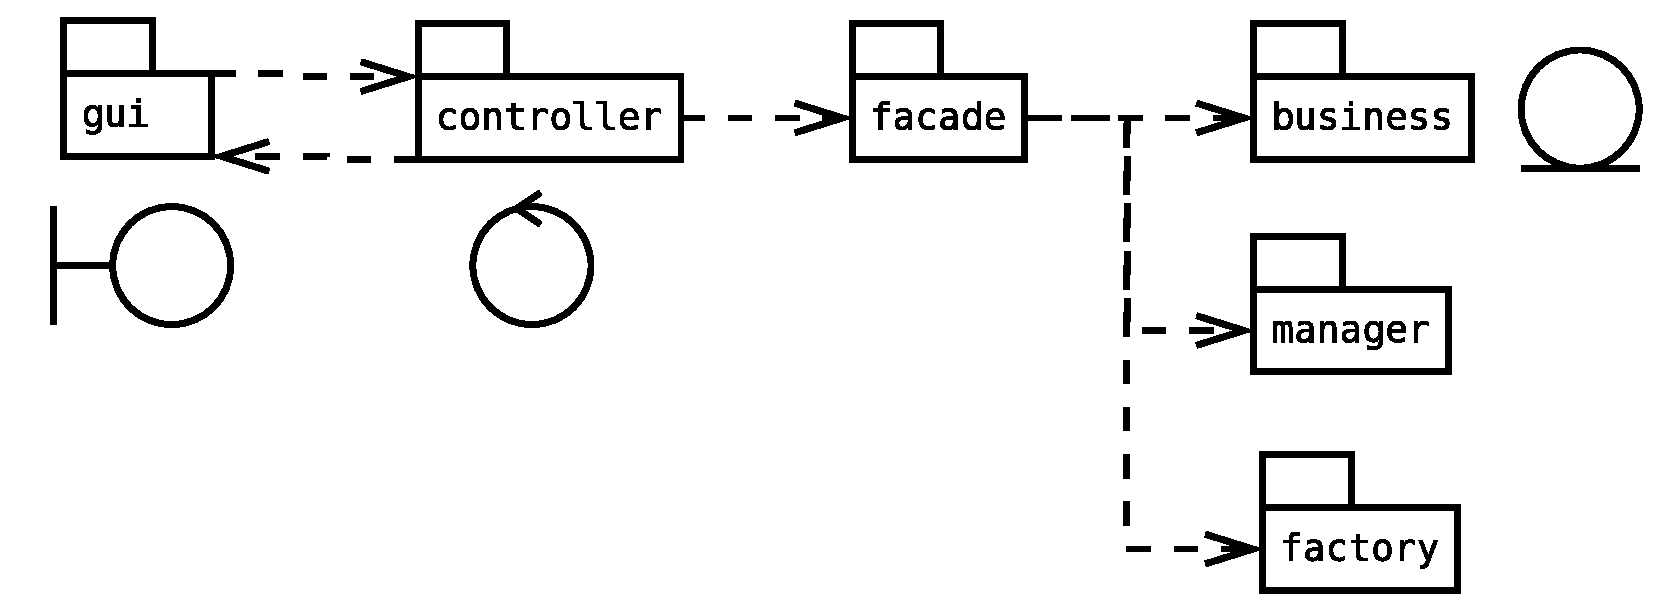
\includegraphics[width=14cm]{images/paquetage.eps}
  \caption{Diagramme de paquetage de l'application.}
  \label{diagramme_de_paquetage_idb}
\end{figure}

\subsection{Couche présentation}
La couche \textit{présentation} contient les IHM de l'application.
Le code des classes ne contient que ce qui est nécéssaire pour l'agencement et le paramétrage des composants sur la vue.

Sur la figure \ref{diagramme_de_paquetage_idb}, la couche présentation se trouve dans le paquetage \textit{gui} (Graphic User Interface, IHM en français).

\subsection{Couche contrôle}
La couche \textit{contrôle} contient l'\textit{intelligence} des IHM, c'est à dire ce qu'il doit se passer \textbf{hors} de la vue (dans les bases de données, la RAM etc.) après un clic sur tel ou tel bouton, case à cocher ou tout autre composant.

Cette couche décharge le code des IHM et fait office d'\textit{indirection} entre les vues et le reste de l'application : les IHM ne connaissent que leurs contrôleurs respectifs.

Sur la figure \ref{diagramme_de_paquetage_idb}, la couche contrôle se trouve dans le paquetage \textit{controller}.
Comme le montre le diagramme, les dépendances entre les paquetages \textit{gui} et \textit{controller} ne sont pas unilatérales.
C'est trompeur : en réalité, les contrôleurs connaissent leurs IHM uniquement pour éviter de les afficher en double.
Il était possible de faire des IHM des \textit{singletons}, cependant cela n'aurait pas réglé le défaut du \textit{fort couplage}.

Les IHM ne sont donc pas des singletons et les contrôleurs y sont associés (au sens UML du terme).

\subsection{Couche entité}
La couche \textit{entité} ou \textit{métier} contient la valeur ajouté de l'application, c'est à dire toutes les classes dont le code génère le service de l'application.

Dans ce projet tuteuré, les classes métiers sont une pseudo-couche \gls{orm}
\footnote{\label{faux_orm}Les ORM convertissent les données en objets, dans cette application se sont les \textit{conteneurs} des données qui sont convertis en objets.}
qui représentent les tables et les contraintes du SGBD connecté à l'application.
Elles limitent les accès réseaux au SGBD, ce qui augmente les performances de l'application, et participent à la génération de code SQL à partir des saisies faites dans les IHM.

Sur la figure \ref{diagramme_de_paquetage_idb}, la couche métier se trouve dans le paquetage \textit{business}.

\subsection{Couche facade}
La couche \textit{facade} reprend le \textit{design pattern} façade.
Son utilité est de limiter les dépendances entre les contrôleurs et les autres paquetages de l'application.
Elles n'apportent rien d'autres à l'application.

Sur la figure \ref{diagramme_de_paquetage_idb}, la couche facade se trouve dans le paquetage \textit{facade}.

Les figures \ref{trois_premières_couches} et \ref{facades_et_managers} montrent les intéractions entre les façades et les paquetages dont elles cassent les dépendances avec les contrôleurs. Les couleurs sont indépendantes d'une figure à l'autre, elles distinguent :
\begin{itemize}
\item les couches présentation, contrôle et façade sur la figure \ref{trois_premières_couches},
\item les associations entre les façaces et les autres classes sur la figure \ref{facades_et_managers}.
\end{itemize}

\begin{figure}[!h]
\centering
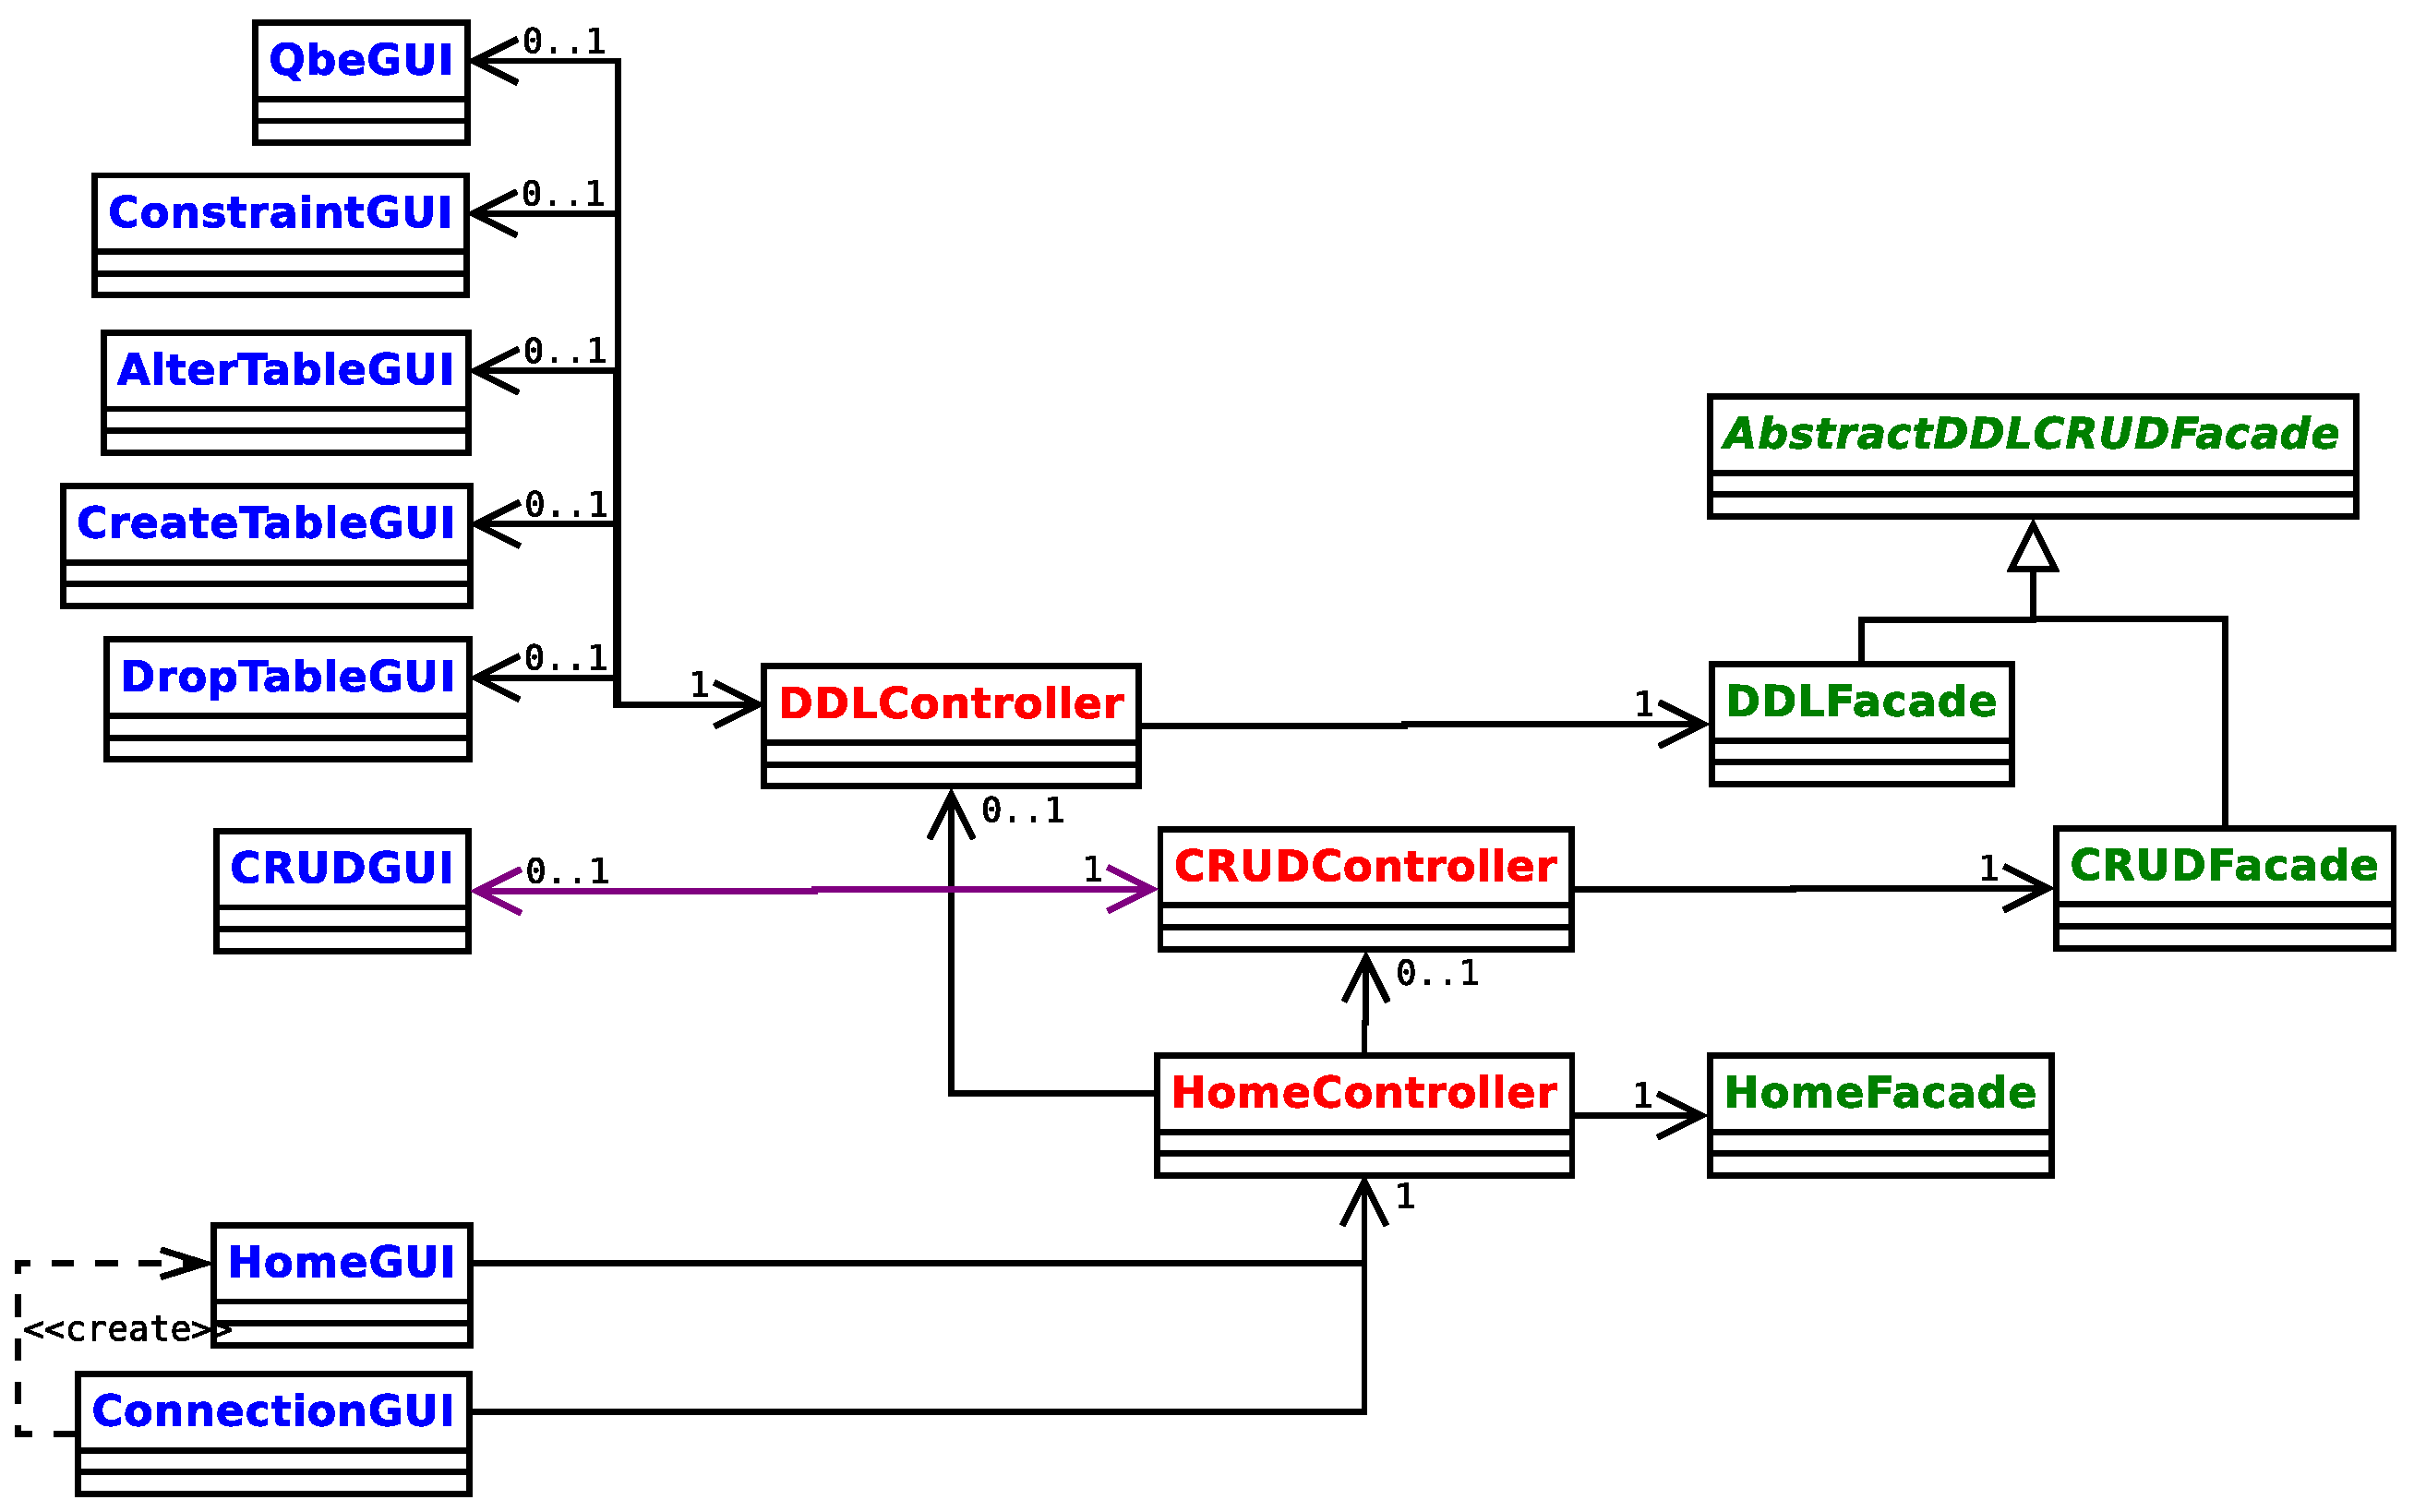
\includegraphics[width=14cm]{images/facades_crud_ddl.eps}
\caption{Couches présentation, contrôleur et façade.}
\label{trois_premières_couches}
\end{figure}

\begin{figure}[!h]
\centering
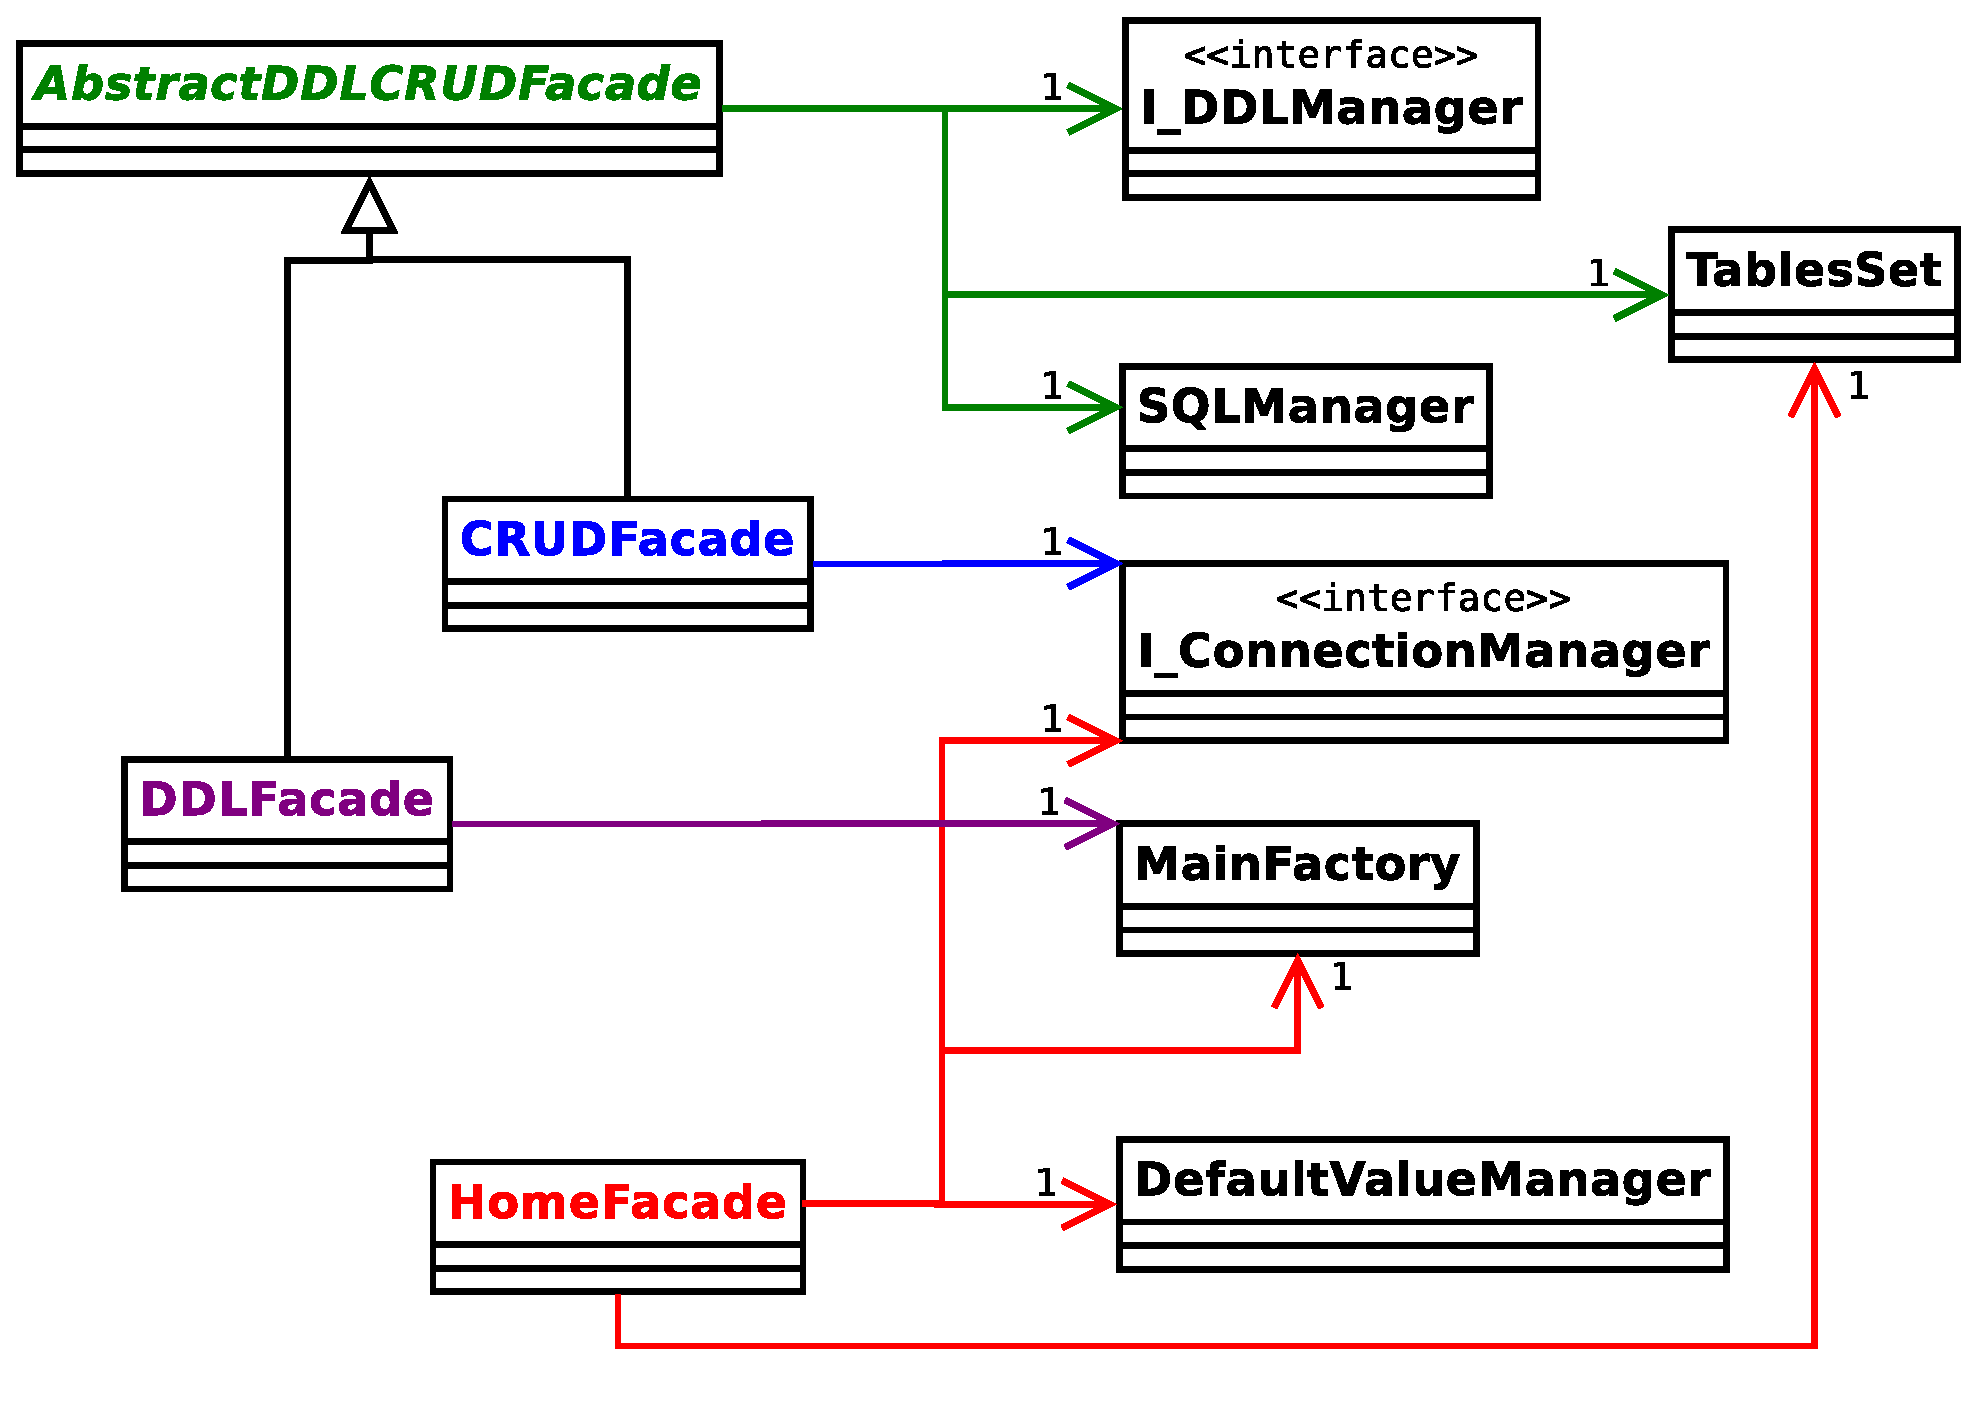
\includegraphics[width=14cm]{images/facades_managers.eps}
\caption{Intéractions entre les façades et les autres paquetages.}
\label{facades_et_managers}
\end{figure}

\subsection{Couche DAO}
La couche \gls{dao} permet d'enregistrer et récupérer des informations depuis le SGBD.
En temps normal, les DAO permettent d'enregistrer des données.
Dans cette application, ils permettent d'enregistrer les données, leurs conteneurs (tables) et les \glspl{constraint}.
Ils ont également un rôle de générateur de code SQL, généralement "simple" et qui diffère selon le SGBD connecté, contrairement aux classes métiers qui fournissent du SQL qui fonctionne sur tous les SGBD.

Sur la figure \ref{diagramme_de_paquetage_idb}, la couche DAO se trouve dans le paquetage \textit{manager}.
Les DAO sont utilisés \textit{à peu près} en suivant le design pattern \textit{data mapper}
\footnote{\label{faux_data_mapper}Ce pattern stipule que ce soient les classes qui \underline{utilisent} les \gls{orm} qui les enregistrent dans un système de stockage.}
, dans le sens où ce sont les contrôleurs de l'application qui les utilisent (par le biais des façades) pour enregistrer les tables et ce qu'elles contiennent.




\section{Paquetages}
Cette section détaille les couches évoquées dans l'autre section \ref{partie_architecture} et complète sur les paquetages \textit{factory} (visible sur la figure \ref{diagramme_de_paquetage_idb}) et \textit{useful}.

\subsection{Paquetage des fabriques}
L'application utilise une \textit{fabrique abstraite} qui se trouve dans le paquetage \textit{factory}.

\subsubsection{Utilité}
L'une des problématiques est de faire fonctionner l'application avec tous les \glspl{sgbd} disponibles.
Bien que le langage \gls{sql} soit normé, les SGBD ne l'implémentent pas de la même manière, ce qui veut dire que la syntaxe des requêtes est \underline{différente} d'un SGBD à l'autre.
Ce point constitue la difficulté principale du développement, et la fabrique abstraite permet de la régler tout en respectant les principes \textit{ouvert/fermé}. Elle permet également de régler d'autres problèmes mineurs, comme la gestion de la casse qui diffère d'un SGBD à l'autre
\footnote{\label{casse_et_sgbd}Oracle convertit le nom des tables et contraintes en majuscule, ce qui n'est pas le cas de MySQL par exemple.}.

En raison du temps disponible pour le développement, l'application ne fonctionne qu'avec les SGBD Oracle et MySQL.
En revanche, elle accueille un nouvel SGBD sans \textbf{modifier} le code existant: il faut seulement en \textbf{ajouter}. %pas de u après le e pour accueille

\subsubsection{Dépendances supplémentaires}
Les dépendances de ce paquetage ne sont pas toutes représentées sur la figure \ref{diagramme_de_paquetage_idb}.
Le diagramme montre que la fabrique est toujours appelée depuis un contrôleur (par le biais d'une façade).
En plus de cette dépendance, d'autres de stéréotypes \textit{create} existent :
\begin{itemize}
\item vers le paquetage \textit{gui}, pour que les \glspl{ihm} utilisent une stratégie de saisie différente en fonction du \glspl{sgbd} (gestion de la casse par exemple),
\item vers le paquetage manager, pour que le code \gls{sql} généré ait la syntaxe du SGBD connecté.
\end{itemize}

\subsubsection{Statique de la fabrique}
\begin{figure}[!h]
  \centering
  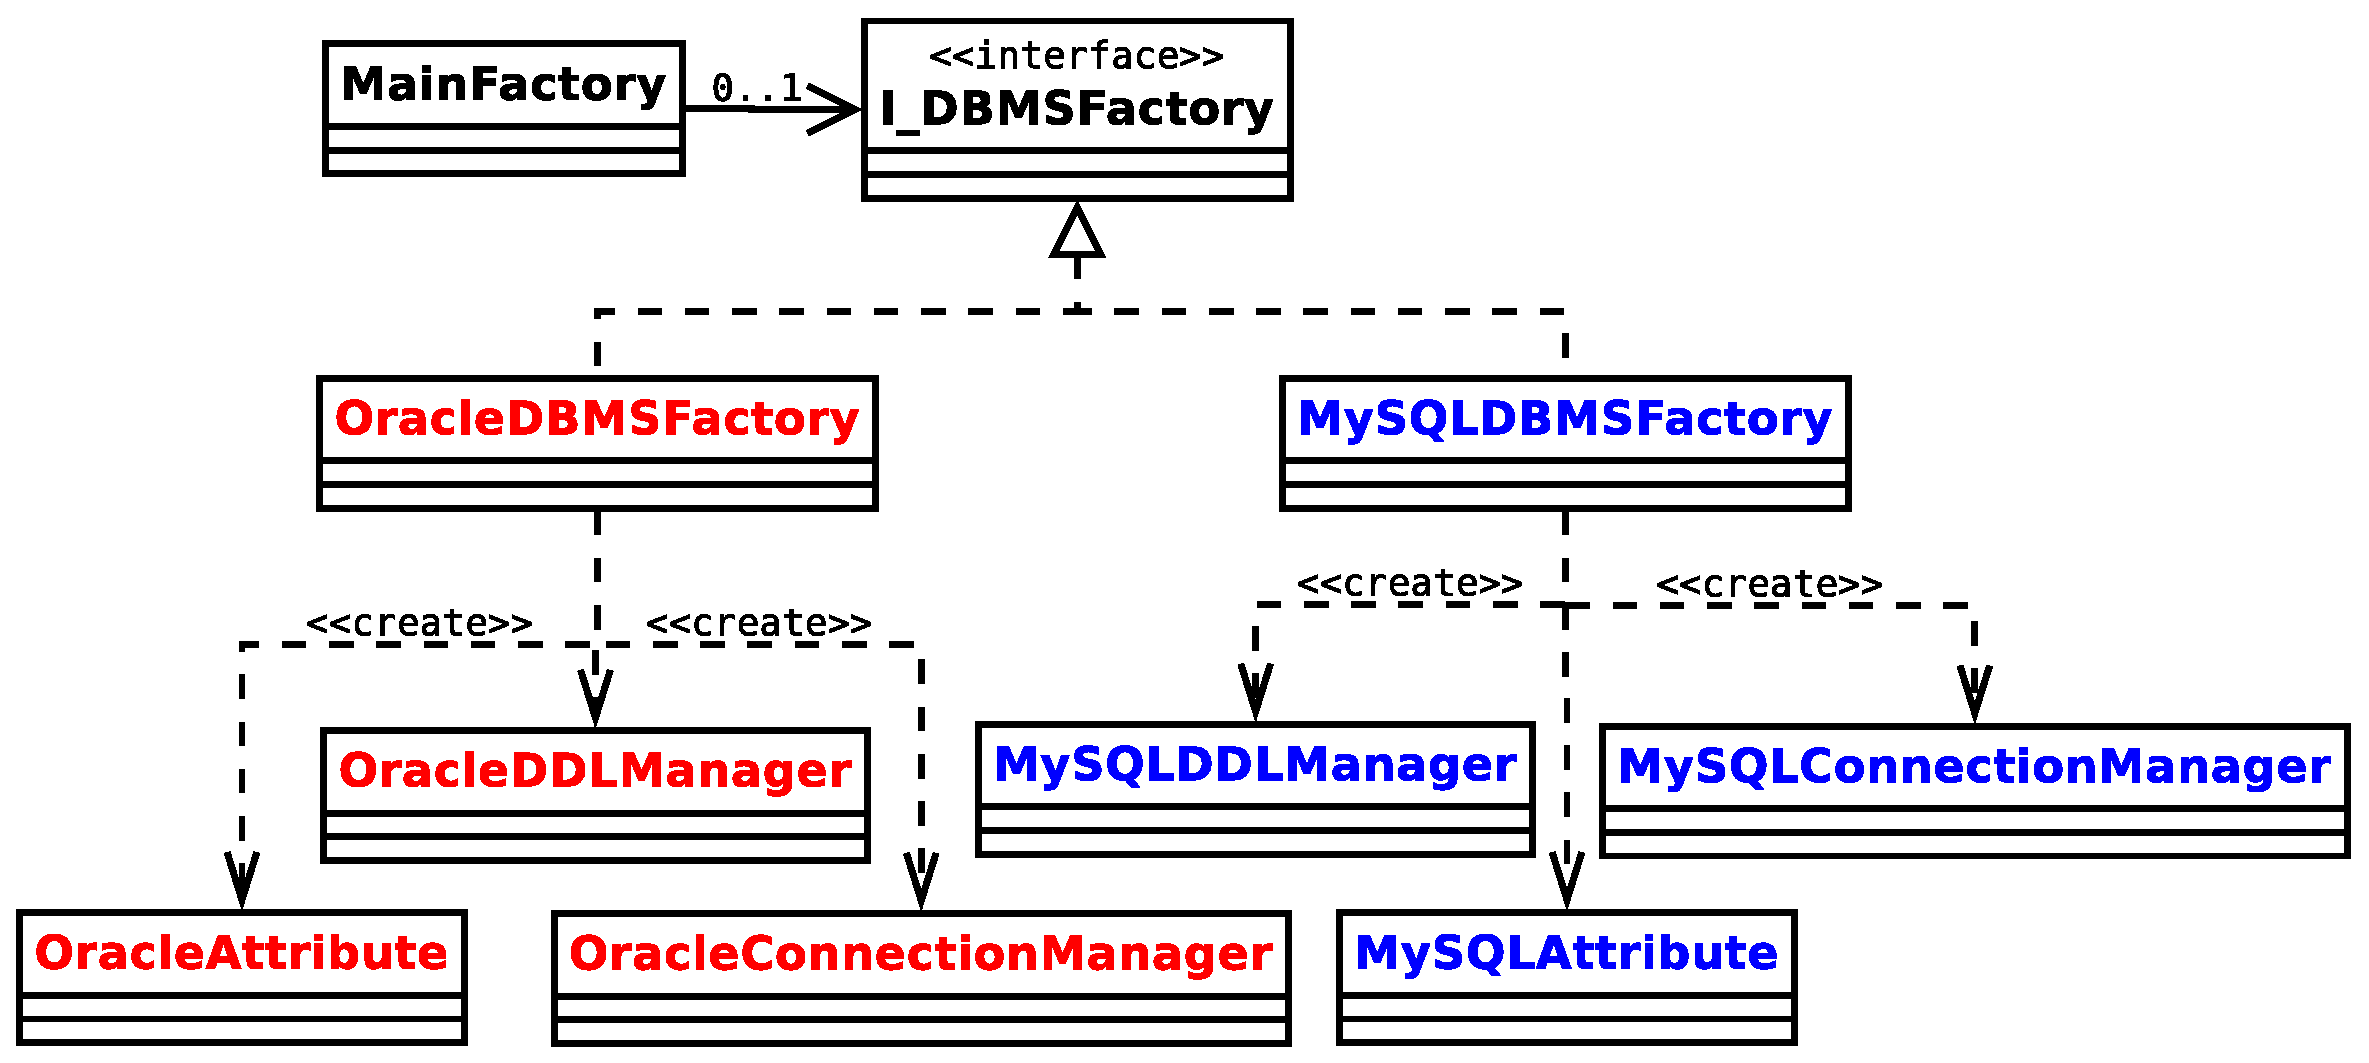
\includegraphics[width=14cm]{images/diagramme_classes_fabriques.eps}
  \caption{Fabrique abstraite de l'application.}
  \label{diagramme_classes_fabrique}
\end{figure}

Sur la figure \ref{diagramme_classes_fabrique}, la classe \textit{MainFactory} est une fabrique concrète de fabriques abstraites.
Elle s'associe avec une \textit{I\_DBMSFactory} qui représente le SGBD connecté pour créer les bons objets, ce qui correspond à un pattern \textit{stratégie}.

La seule fabrique de l'application est MainFactory.
Pour ajouter un nouvel SGBD, il faut créer une classe qui implémente l'interface I\_DBMSFactory, donc \textbf{ajouter} du code.
La seule \textbf{modification} nécessaire se trouve dans MainFactory, pour qu'elle puisse instancier l'implémentation.

\subsection{Paquetage des outils}
Plusieurs classes sont utilisées un peu partout dans le code.
Ces classes (développées par l'équipe du projet) sont regroupées dans le paquetage \textit{useful}, qui n'apparaît pas sur la figure \ref{diagramme_de_paquetage_idb}.

\subsubsection{Dépendances}
Tous les paquetages de cette application dépendent du paquetage useful, mais ce n'est pas gênant dans la mesure où le code de ces classes n'est jamais amené à changer.
Ce paquetage peut être comparé à \textit{java.util}
\footnote{\label{paguetage_java_util}Package \textit{java.util} : \url{https://docs.oracle.com/javase/7/docs/api/java/util/package-summary.html}}
de java, qui contient les utilitaires que l'on retrouve dans toutes les applications.

\subsubsection{Classe Response}
\begin{figure}[!h]
  \centering
  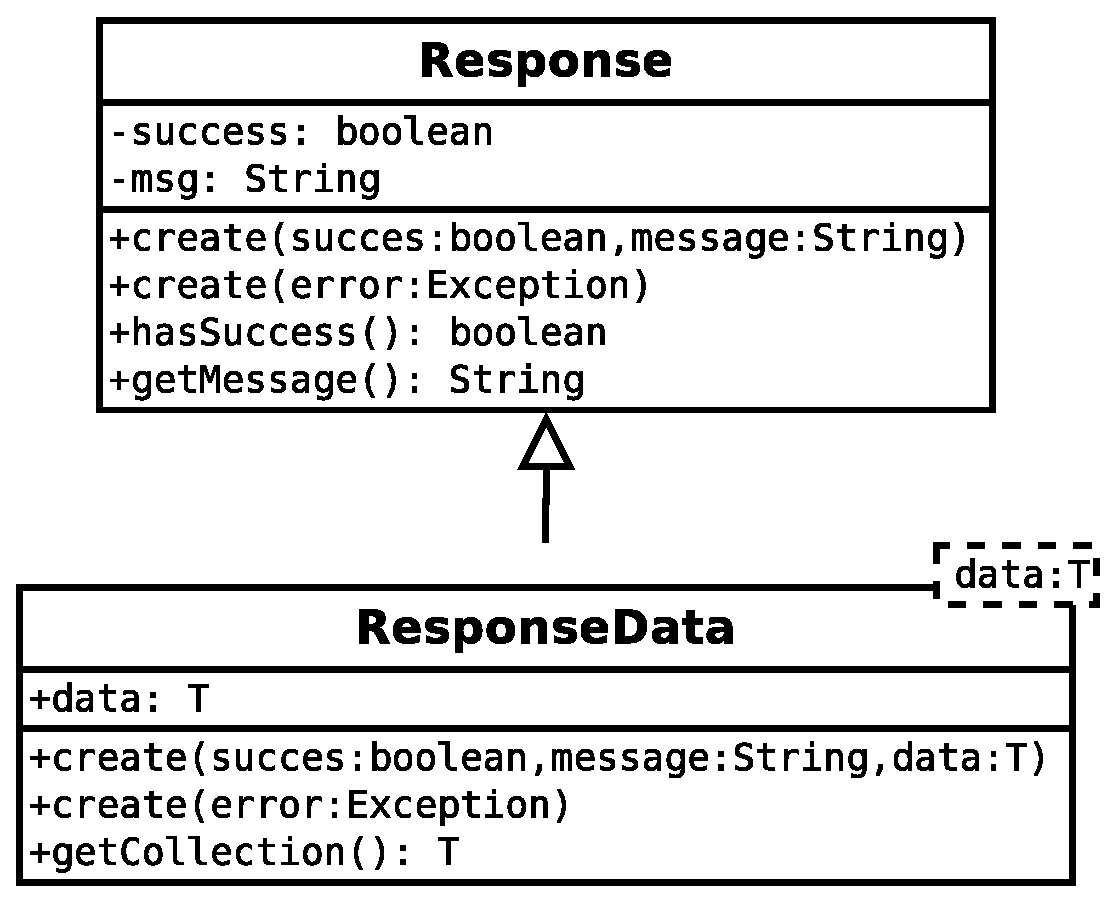
\includegraphics[width=10cm]{images/response.eps}
  \caption{La classe Response en mode plan.}
  \label{uml_classe_response}
\end{figure}

Les DAO de l'application utilisent les packages \textit{java.sql} et \textit{javax.sql}
\footnote{\label{paquetages_sql}Package \textit{java.sql} : \url{https://docs.oracle.com/javase/7/docs/api/java/sql/package-summary.html}}.
En cas de problèmes lors du dialogue avec les SGBD, les méthodes de ces packages lèvent les exceptions \textit{SQLException}.

Travailler avec les exceptions est pénible : elles forcent à utiliser des clauses \textit{try/catch} où à déclarer des méthodes qui lèvent des exceptions.
La programmation devient chaotique puisqu'elle se rapproche d'une programmation événementielle, la ligne d'exécution peut sauter à tout moment pour se retrouver dans la clause catch.
Il faut ensuite gérer les types de retour des méthodes ou les exceptions levées.

Dans ce projet, les exceptions restent bloquées dans les classes du paquetage manager.
Les méthodes retournent des objets \textit{Response} et ne lèvent aucune exception.

Cette classe possède deux attributs, comme le montre la figure \ref{uml_classe_response}:
\begin{enumerate}
\item un booléen, vrai si et seulement si la méthode du DAO a réussi,
\item une chaîne de caractère qui contient un message du SGBD si la méthode du DAO a échouée, ou un message de réussite si tout c'est bien passé.
\end{enumerate}

Avec Response, on récupère donc deux informations en un seul \textit{return}.
Les succès ou les échecs des appels au SGBD sont traités uniquement dans instructions conditionnelles.

Ces objets sont utilisés également dans les IHM : une Response dont le premier attribut est faux affiche un message rouge d'erreur.
Une Response positive affiche un message bleu.

\subsubsection{Classe ResponseData<T>}
La classe Response est spécialisée par ResponseData.
Elle est utile lorsque le DAO est utilisé pour \textbf{récupérer} des informations du SGBD.
En plus des informations de la classe Response, elle possède une collection d'objets T.
Elle peut par exemple stocker le résultat d'une requête SELECT ou encore retourner le nom des tables disponibles dans la base de données.

\subsection{Paquetage des IHM}
Les IHM sont regroupées dans le paquetage \textit{gui}.

\subsubsection{Diagramme de classes des IHM}
\begin{figure}[!h]
\centering
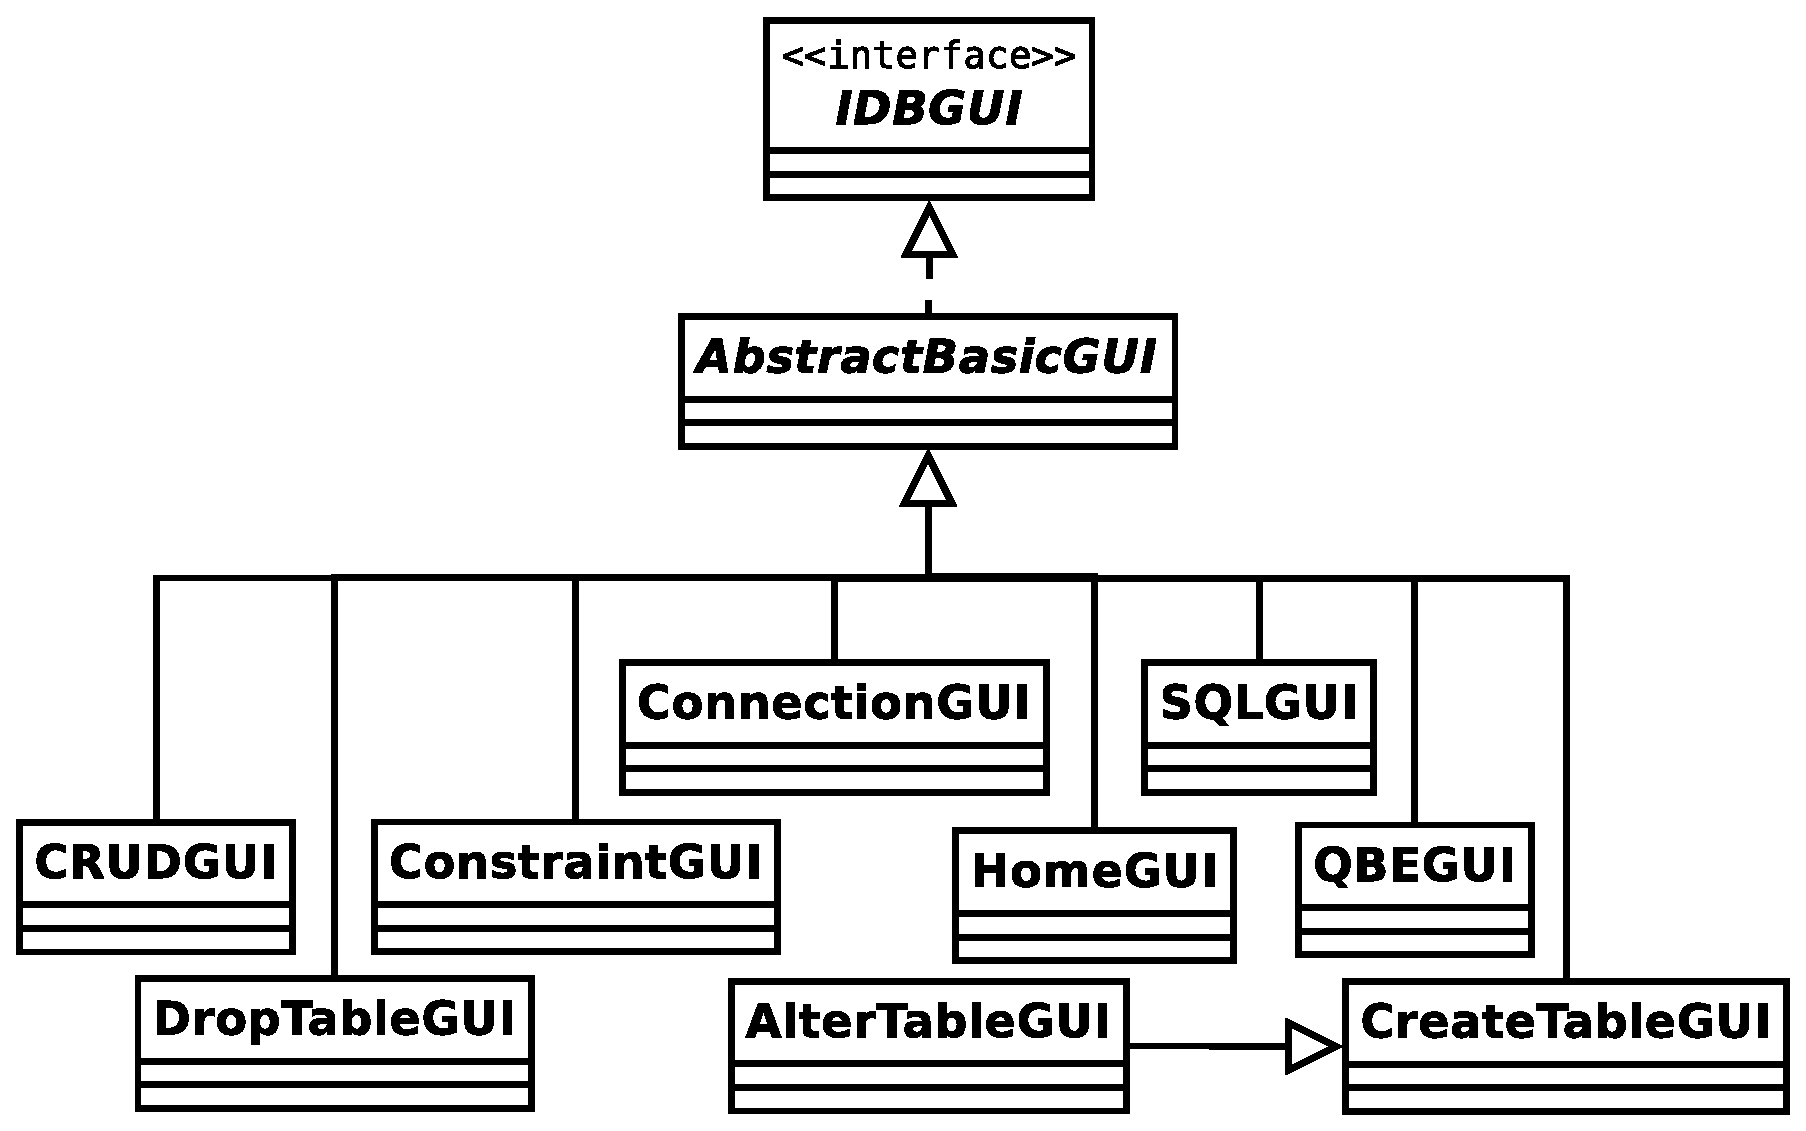
\includegraphics[width=14cm]{images/gui.eps}
\caption{Les IHM spécialisent \textit{AbstractBasicGUI}.}
\label{hierarchie_des_ihm}
\end{figure}

AbstractBasicGUI regroupe un ensemble de méthodes qui gèrent seules l'agencement des composants
\footnote{\label{composants_ihm}Barre de défilements, case à cocher, étiquettes, boite saisie etc.}
, ce qui permet de concevoir une IHM en se focalisant sur le fond plutôt que sur la forme.

\subsubsection{Comportement commun}
Les IHM utilisent les méthodes suivantes :
\begin{itemize}
\item \textit{talk()}, qui communique avec l'utilisateur en écrivant un message sur une étiquette située \textbf{en haut} de la fenêtre,
\item \textit{isComplete()}, qui autorise à appuyer sur le bouton "final" d'une IHM si et seulement si toutes les informations sont remplies.
\end{itemize}

En généralisant le comportement des IHM, l'utilisateur prend des habitudes sur l'application, ce qui la rend plus ergonomique.

\subsection{Paquetage des gestionnaires}
Le paquetage \textit{manager} regroupe les DAO et d'autres outils.
Tout le contenu n'est pas détaillé dans cette sous-section.

Les gestionnaires sont \textit{développés pour des interfaces} , afin de respecter le principe \textit{ouvert/fermé} et de permettre à l'application de se connecter à n'importe quel SGBD.
Les objets sont instanciés depuis la fabrique MainFactory.

\subsubsection{Gestionnaires de connexion}
Les méthodes de connexions varient d'un SGBD à l'autre avec le \gls{JDBC}.
Par conséquent, les classes qui gèrent la connexion implémentent une interface \textit{I\_ConnectionManager} (figure \ref{connection_managers_uml}).

\begin{figure}[!h]
\centering
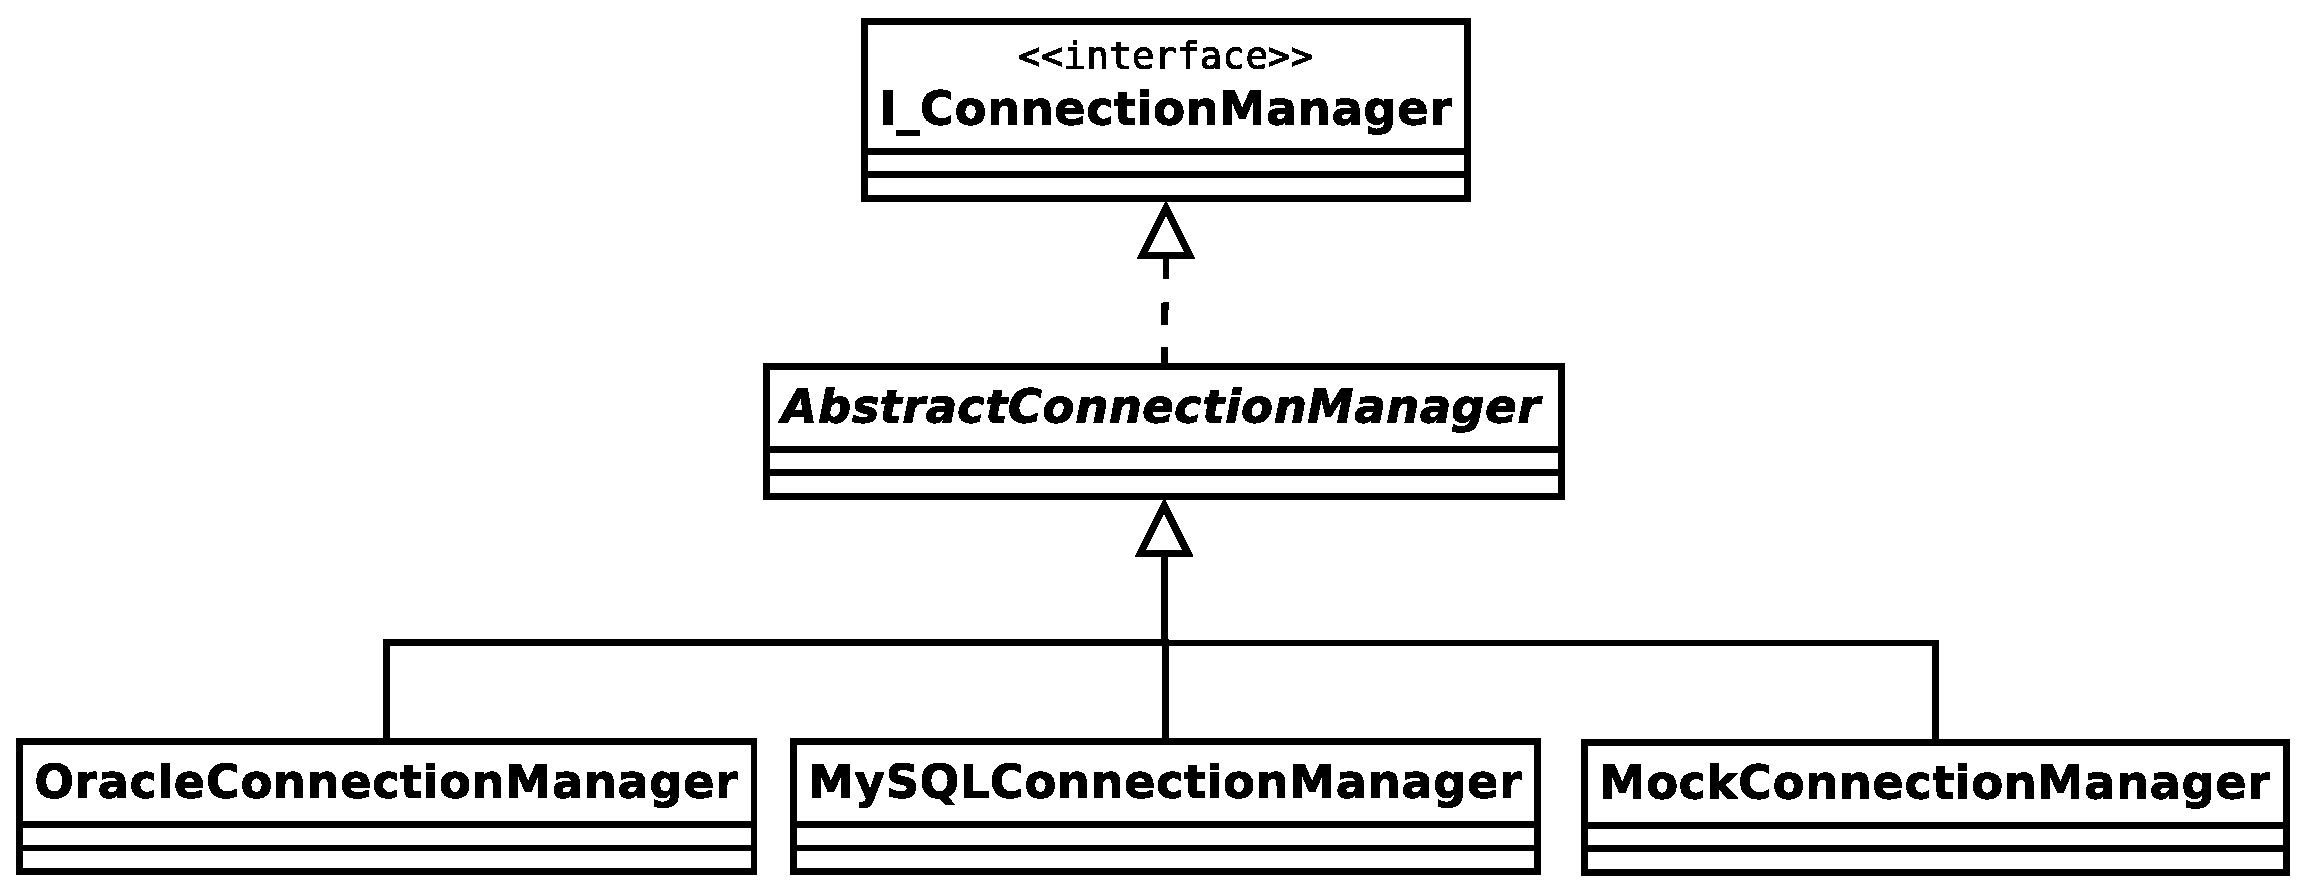
\includegraphics[width=14cm]{images/connection_managers.eps}
\caption{Implémentations du I\_ConnectionManager.}
\label{connection_managers_uml}
\end{figure}

\subsubsection{Gestionnaires de définition des données}
Les gestionnaires de définition des données sont développés pour une interface \textit{I\_DDLManager} afin de générer les requêtes SQL de LDD compatibles avec le SGBD connecté (figure \ref{ddl_managers_uml}).

\begin{figure}[H]
\centering
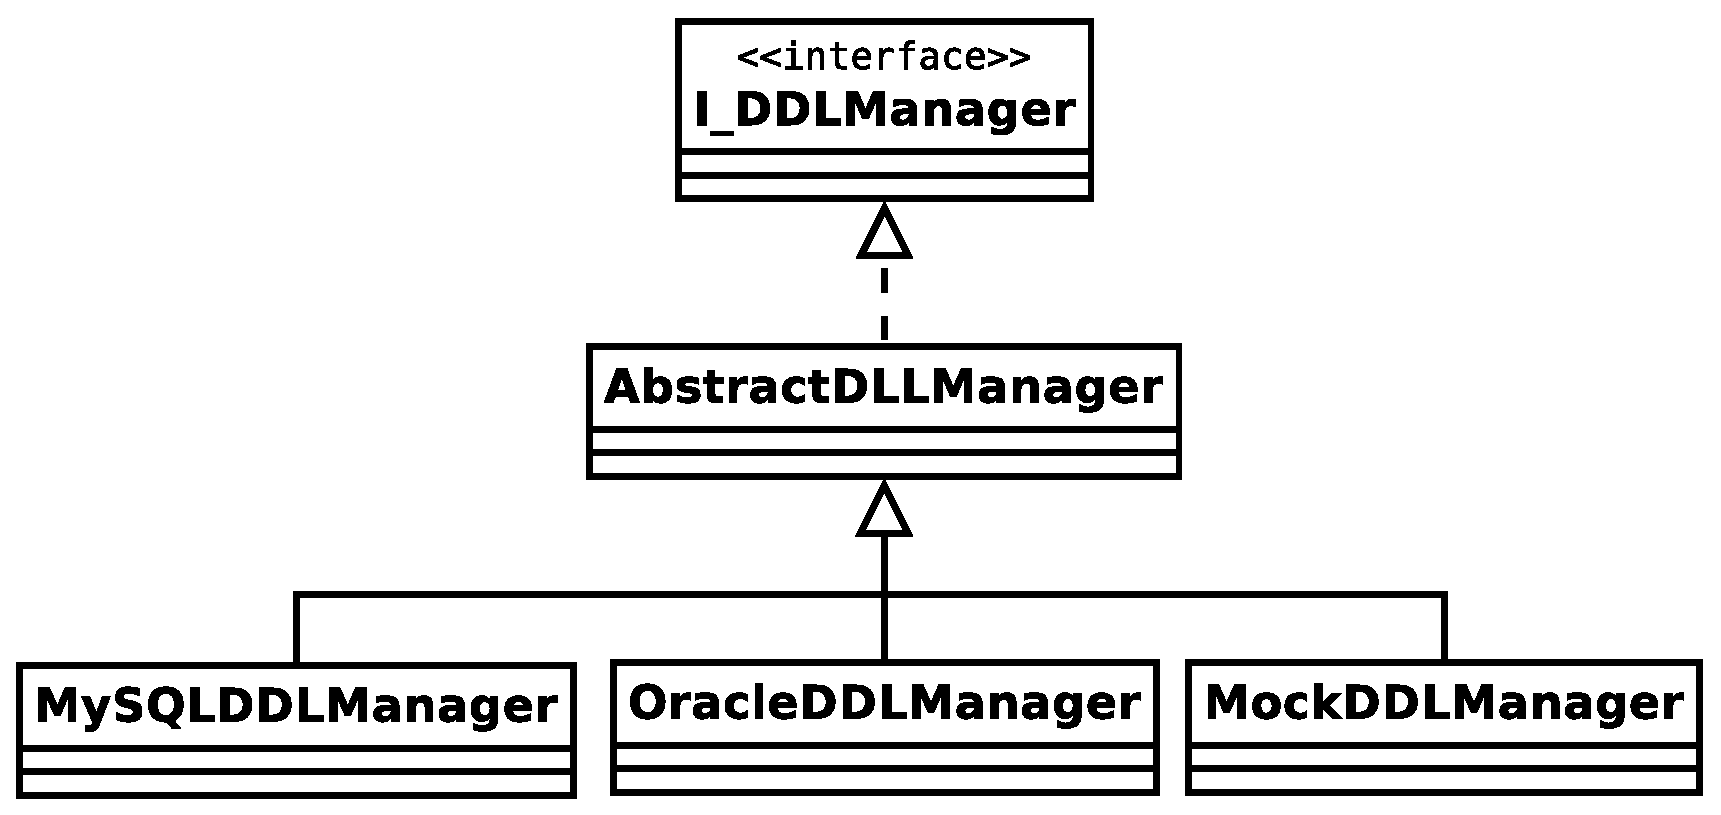
\includegraphics[width=14cm]{images/ddl_managers.eps}
\caption{Implémentations du I\_DDLManager}
\label{ddl_managers_uml}
\end{figure}


\section{Les classes métiers}
Il nous a été nécessaire de créer des classes métiers représentant fidèlement le comportement réel des tables contenues dans n'importe quel \sgbd

\begin{figure}[!h]
\centering
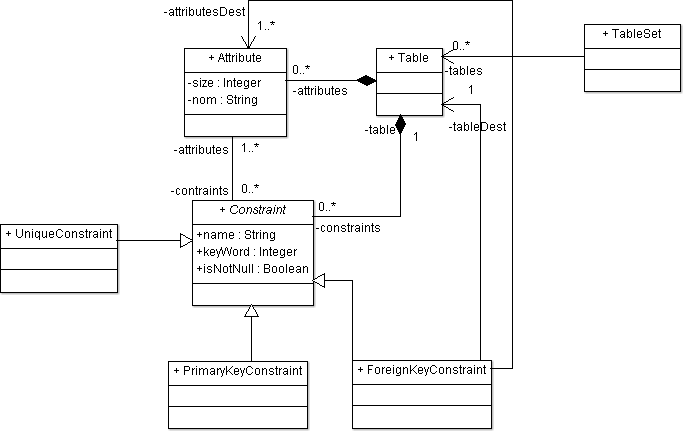
\includegraphics[width=18cm]{images/metier.png}
\caption{Diagramme de classes métiers}
\label{classes_metiers}
\end{figure}


Ces classes ont une particularité, elles peuvent générer du code SQL à partir de leurs attributs ou de différents arguments.
Lorsqu'une table est supprimé, tous les attributs de la table sont détruits et toutes les contraintes composant les attributs et la table sont détruit également.
Si un seul attribut est détruit, toutes les contraintes qui le compose sont détruites, ainsi, une contrainte \textbf{ForeignKeyConstraint} sera détruit même si elle concerne un second attribut.
\exemple{Une fk1 est composé de att1 et att2 pointant sur pk1 et pk2 respectivement.
\newline Si l'on supprime att1, alors la clé étrangère ne peut plus respecter la norme et la contrainte fk1 est détruite.}
\label{section_metiers}




\chapter{Les Tests}
Les tests constituent des éléments indispensables, ils permettent d'avancer sur un projet sans que les nouvelles implémentations ne viennent modifier le comportement existant.
\section{Pourquoi tester}


Idéalement, chaque classe devrait être testée \textbf{unitairement}.
Malheureusement, certains comportement ne peuvent pas être testés  de façon automatique. Par exemple, pour tester les fonctionnalités d'un logiciel ayant des interactions avec \gls{sgbd}, il faudrait que l'utilisateur stocke ses identifiants de connexion en dur dans une classe accessible par sa classe de test, et il faudrait également qu'il ait préalablement créé manuellement la liste de toutes les tables nécessaires au fonctionnement de son programme.
\bigbreak

Pour pallier à ce problème, il est possible de créer une classe mock avec des comportements précis directement introduits par le développeur. Si la classe normale doit effectuer une vérification sur un système externe et retourner \textit{true} ou \textit{false} selon le résultat de cette vérification, la classe mock, elle, retournera directement \textit{true} ou \textit{false} sans faire de vérifications, c'est ce que l'on appelle "\underline{mocker la classe}"). L'inconvénient de cette façon de faire est que cela agrandit considérablement le nombre de classes Java du projet.


\bigbreak
  Heureusement, il existe des bibliothèques externes qui permettent de créer des objets \gls{mock}* sans avoir à créer une nouvelle classe.
Les classes natives de Java ne seront pas "mockés" car celles-ci ont déjà été testées avant d'être intégrées à Java et sont donc considérées "sans bugs".
\bigbreak
Exemple d'utilisation de la bibliothèque externe \textit{Mockito} :

\lstset{
language=Java,
basicstyle=\normalsize, % ou ça==> basicstyle=\scriptsize,
upquote=true,
aboveskip={1.5\baselineskip},
columns=fullflexible,
showstringspaces=false,
extendedchars=true,
breaklines=true,
showtabs=false,
showspaces=false,
showstringspaces=false,
identifierstyle=\ttfamily,
keywordstyle=\color[rgb]{0,0,1},
commentstyle=\color[rgb]{0.133,0.545,0.133},
stringstyle=\color[rgb]{0.627,0.126,0.941},
}
\begin{lstlisting}
SQLManager sqlManager = Mockito.mock(SQLManager.class);

Mockito.when(sqlManager.sendQuery(Mockito.contains("SELECT"))).thenReturn(true);
Mockito.when(sqlManager.sendQuery("")).thenThrow(IllegalArgumentException.class);
Mockito.when(sqlManager.getGeneratedJTable()).thenReturn(new JTable());
Mockito.when(sqlManager.getGeneratedReply()).thenReturn(Mockito.anyString());

\end{lstlisting}
\bigbreak

Il est utile de tester pour vérifier que les fonctionnalités telles que définies dans le cahier des charges correspondent bien à celles qui ont été développées.
\exemple{Un utilisateur doit pouvoir se connecter à la base de données. Si un jour, après une légère modification, l'utilisateur ne peut plus se connecter alors qu'il le devrait, le reste du logiciel deviendrait inutile aux yeux du client\newline}

Certaines classes ne sont pas testables sans utiliser des bibliothèques complexes nécessitant d'écrire de nombreuses de lignes de code pour tester une seule fonctionnalité. C'est le cas notamment des classes servant d'IHM et dont la seule façon possible de tester est d'implémenter un objet dit "Robot" qui simulera l'action d'un utilisateur humain. Après concertation avec le tuteur du projet il a été décidé que ces tests se feront manuellement.

\section{Les tests choisis}

Nous avons donc choisis de tester en priorité les classes \textbf{Métiers}, une suite de tests appelés \textbf{AllTests} se charge  de lancer tous les tests liés aux classes métiers :
\\

\begin{itemize}
	\item testAttribute
	\item testTable
	\item testConstraint
	\item testTableSet
\end{itemize}

\textit{Voir section \ref{section_metiers} traitant des classes métiers}
\\


La plupart des tests ont été écrits après l'implémentation des fonctionnalités sauf certaines classes utilisant les classes du package \textbf{Métiers} qui ont été développés en \gls{tdd}*.
\medbreak
La classe faisant office de \gls{dao}* pour le \gls{crud} utilise une bibliothèque externe pour pouvoir mocker son comportement : \textbf{Mockito}. Tous les appels à cette classe sont donc capturés et gérés par le développeur directement dans la classe de test une fois celle-ci "mocké", ce qui permet de tester sa couche de contrôle et sa couche de façade sans créer de classes de \gls{mock} supplémentaires.

\medbreak

Les structures de données ResponseData et Response servant à éviter de traiter des exceptions \textit{(voir Figure  \ref{uml_classe_response})} sont également testés individuellement, leur place étant importante au sein du projet.

\bigbreak
Des tests sur la connexion sont également effectués, c'est l'un des éléments clés du projet car toutes les fonctionnalités reposent sur le fait que la connexion est fonctionnelle. Les tests d'intégrations ne passent pas si les tests unitaires de la connexion ne passent pas).

Pour cela, différents objets nécessaires à l'établissement d'une connexion ont été \textit{mockés} et des tests vérifiant l'état de la connexion sont effectués.




\chapter{Manuel d'utilisation}
L'application se lance lors d'un double clique sur l'exécutable.

\section{Se connecter}
La première fen\^etre à apparaitre est l'interface de connexion ci-dessous :
\begin{figure}[!h]
\centering
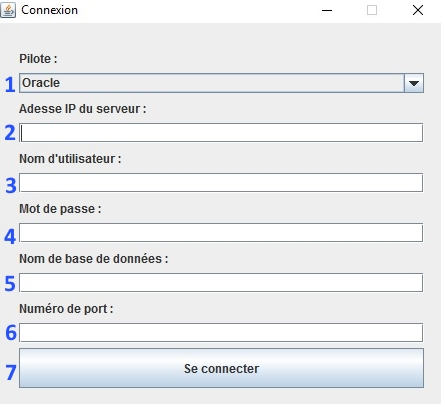
\includegraphics[width=10cm]{./images/manuel/se_connecter.jpg}
\caption{IHM - Se connecter}
\label{se_connecter}
\end{figure}

Afin de se connecter il faut renseigner les différents champs présents dans la fen\^etre.

\begin{enumerate}
\item choix du SGBD* (Oracle, MySQL).
\item Adresse IP du serveur ou est stockée votre base de données.
\item Nom d'utilisateur utilisé pour vous connecter à votre base de données. 
\item Mot de passe utilisé pour vous connecter à votre base de données.
\item Nom de la base de données.
\item Numéros de port du serveur ou est stockée votre base de données.
\item Cliquer sur le bouton \textbf{se connecter} pour tenter de se connecter au serveur.
\end{enumerate}

Connexion aux serveurs de l'IUT si vous \^etes étudiant :\\

\textbf{Oracle}
\begin{itemize}
\item SGBD : Oracle
\item Adresse IP : 162.38.222.149
\item Nom d'utilisateur : <nom-de-famille><première-lettre-du-prenom>
\item Mot de passe : <votre-INE>
\item Nom de la base de données : IUT
\item Numéros de port : 1521 \\
\end{itemize}

\textbf{MySQL}
\begin{itemize}
\item SGBD : MySQL
\item Adresse IP : 162.38.222.142
\item Nom d'utilisateur : <nom-de-famille><première-lettre-du-prenom>
\item Mot de passe : <votre-INE>
\item Nom de la base de données : <nom-de-famille><première-lettre-du-prenom>
\item Numéros de port : 3306
\end{itemize}

\section{Créer une table}
Dans le menu principal de l'application, cliquez sur le bouton \textbf{LDD : créer tables} pour ouvrir la fen\^etre de création de tables.

\begin{figure}[!h]
\centering
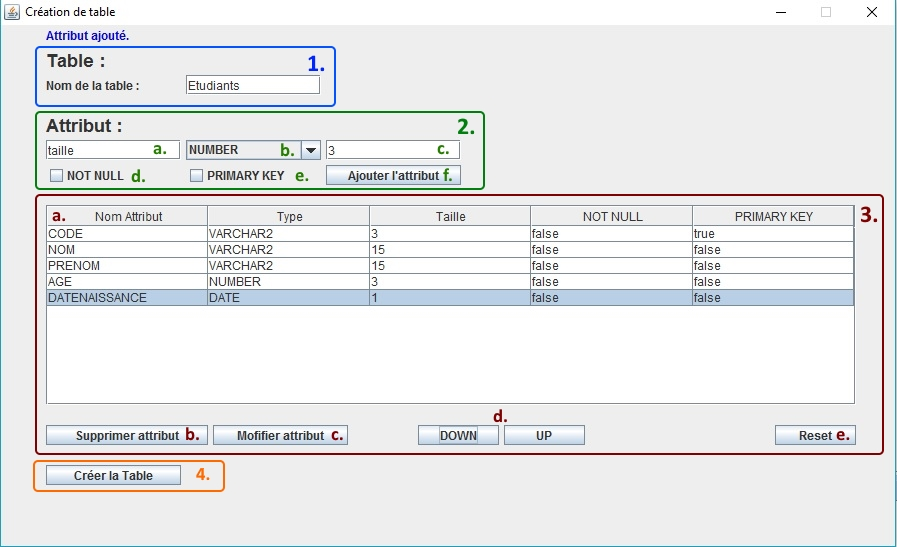
\includegraphics[width=14cm]{./images/manuel/creer_table.jpg}
\caption{IHM - Créer table}
\label{creer_table}
\end{figure}

\begin{enumerate}
\item Nom de ta table - \textit{ex : Etudiants}

\item Gestion des caractéristiques d'un attribut :
\begin{enumerate}
\item Nom - \textit{ex : codeEtudiant}
\item Type - \textit{ex : VARCHAR2}
\item Taille - \textit{ex : 15}
\item A cocher pour que l'attribut ne soit jamais null.
\item A cocher pour que l'attribut soit une clé primaire de votre table.
\item Cliquer sur le bouton \textbf{Ajouter l'attribut} pour tenter d'ajouter un attribut à la table.
\end{enumerate}

\item Gestion des attributs ajoutés :
\begin{enumerate}
\item Tableau contenant les attributs ajoutés avec le bouton <Ajouter l'attribut>.
\item Cliquer sur le bouton \textbf{Supprimer l'attribut} pour supprimer l'attribut sélectionné dans le tableau.
\item Cliquer sur le bouton \textbf{Modifier l'attribut} pour modifier l'attribut sélectionné dans le tableau. 
Les caractéristiques de l'attribut sélectionné sont à modifier dans la zone de gestion des caractéristiques d'un attribut. 
Vous pouvez ensuite valider ou annuler votre modification.
\item Cliquer sur les boutons \textbf{UP/DOWN} pour modifier l'odre des attributs dans le tableau. 
\item Cliquer sur le bouton \textbf{Reset} pour remettre à zéro la fen\^etre de création.
\end{enumerate}

\item Cliquer sur le bouton \textbf{Créer la table} pour tenter la création de la table.
\end{enumerate}

\section{Supprimer une table}
Dans le menu principal de l'application, cliquer sur le bouton \textbf{LDD : supprimer tables} pour ouvrir la fen\^etre de suppression de tables.

\begin{figure}[!h]
\centering
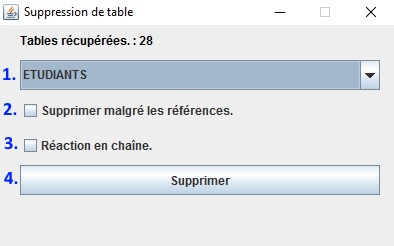
\includegraphics[width=8cm]{./images/manuel/supprimer_table.jpg}
\caption{IHM - Supprimer une table}
\label{supprimer_table}
\end{figure}

\begin{enumerate}
\item Choisir la table à supprimer.
\item A cocher pour supprimer sans prendre en compte les références des autres tables sur celle à supprimer.
\item A cocher pour supprimer la table sélectionnée puis toutes celles qui font référence à cette table et ceci récursivement.
\item Cliquer sur le bouton \textbf{Supprimer} pour tenter la suppression de la table.
\end{enumerate}

\section{Requ\^etes SQL}
Dans le menu principal de l'application, cliquer sur le bouton \textbf{SQL} pour ouvrir la fen\^etre du mode requ\^etes SQL.
\begin{figure}[!h]
\centering
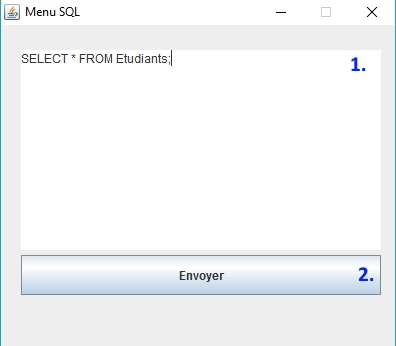
\includegraphics[width=6cm]{./images/manuel/sql.jpg}
\caption{IHM - SQL}
\label{sql}
\end{figure}

\begin{enumerate}
\item Ecrire la requ\^ete dans la zone de saisie - \textit{ex : SELECT * FROM Etudiants;} 
\item Cliquer sur le bouton \textbf{Envoyer} pour tenter d'exécuter la requ\^ete.
Une fenêtre s'ouvre indiquant le résultat de la requ\^ete si la syntaxe est correcte.
\end{enumerate}

\begin{figure}[!h]
\centering
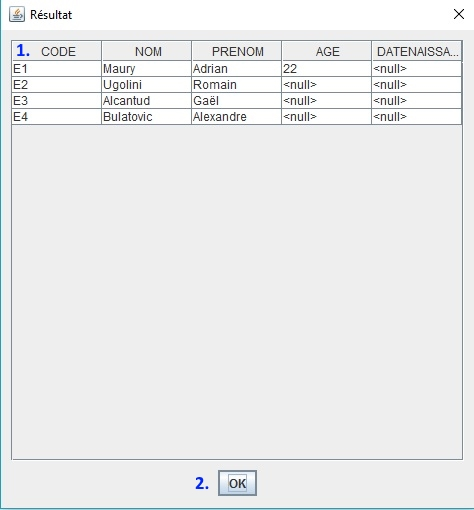
\includegraphics[width=8cm]{./images/manuel/sql_result.jpg}
\caption{IHM - Résultat SQL}
\label{sql_result}
\end{figure}

\begin{enumerate}
\item Résultat de la requ\^ete.
\item Cliquer sur le bouton \textbf{OK} pour fermer la fen\^tre de résultat.
\end{enumerate}

\section{CRUD* les tuples des tables}
Dans le menu principal de l'application, cliquer sur le bouton \textbf{CRUD} pour ouvrir la fen\^etre de gestion des tuples des tables.
\begin{figure}[!h]
\centering
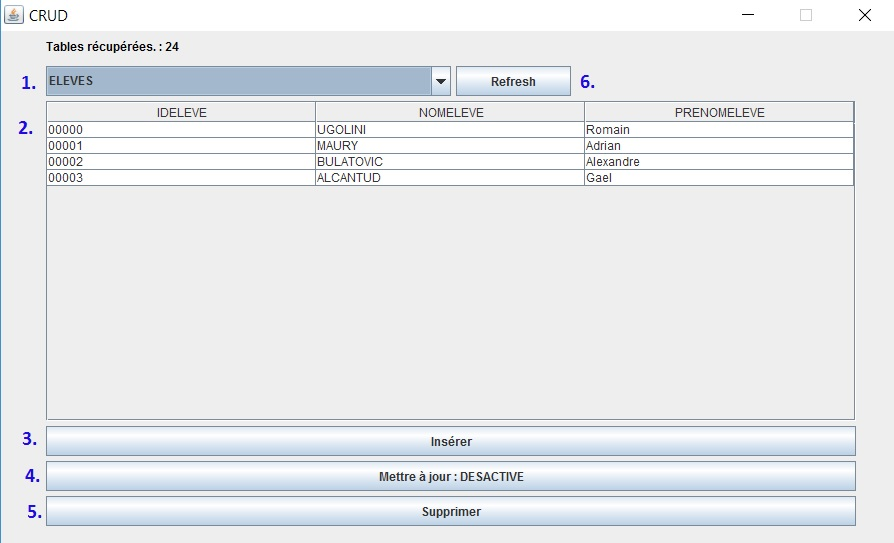
\includegraphics[width=12cm]{./images/manuel/crud.jpg}
\caption{IHM - CRUD}
\label{crud}
\end{figure}

\begin{enumerate}
\item Choisir la table.
\item Tableau contenant les différents tuples de la table sélectionnée.
\item Cliquer sur le bouton \textbf{Insérer} pour ajouter un tuple à la table. Il faut ensuite remplir les informations du nouveau tuple
dans la ligne vide qui s'est ajouté au tableau.
\item Cliquer sur le bouton \textbf{Mettre à jour} pour modifier un tuple de la table. Il faut ensuite modifer les informations du tableau et 
appuyer sur la touche entrée à chaque modification. Quitter le mode modification en cliquant une nouvelle fois sur le bouton \textbf{Mettre à jour}.
\item Cliquer sur le bouton \textbf{Supprimer} pour supprimer le tuple selectionné.
\end{enumerate}

\section{Ajouter et Supprimer des contraintes}


\chapter{Rapport d'activité}
\section{Méthode de developpement}


\subsection{Cycle Itératif}
La méthode de développement pour le projet tuteuré est plus ou moins imposée. En effet pour pouvoir suivre l'avancement du projet, les tuteurs demandent aux étudiants d'utiliser un cycle itératif (figure \ref{cycle_iteratif}).

\begin{figure}[H]
\centering
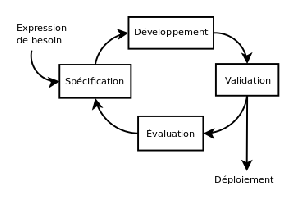
\includegraphics[width=8cm]{images/activite/cycle_iteratif.eps}
\caption{Schéma cycle Itératif}
\label{cycle_iteratif}
\end{figure}

\subsection{Outils de developpement}
Le choix du langage à utiliser était libre, nous avons donc opté pour un langage simple d'utilisation et ayant déjà fait ses preuves : \textbf{Java} (figure \ref{java_logo}).
\\
\\
\\

\begin{figure}[!h]
\centering

\includegraphics[width=8cm]{images/activite/javaLogo.eps}
\caption{Logo Java}
\label{java_logo}
\end{figure}


Nous avons choisi de travailler avec le logiciel \textbf{Éclipse} (figure \ref{eclipse_logo}), l'\gls{IDE} par excellence pour développer du \textbf{Java}.

\begin{figure}[H]
\centering

\includegraphics[width=8cm]{images/activite/eclipseLogo.eps}
\caption{Logo Éclipse}
\label{eclipse_logo}
\end{figure}

\textbf{Éclipse} est agréable à utiliser, il est libre de droits et fait partit des IDE les plus puissants de nos jours.
La bibliothèque nous permettant de faire des \gls{ihm} est swing, une bibliothèque native de Java, constamment mise à jours et très utilisée (donc très documenté).

\section{Planification}
Le projet a été découpé en sept itérations de durée variante (d'une semaine à un mois) en fonction des périodes d'examens et de vacances. Au cours de chaque itérations, de nombreux refactorings de code ainsi que d'organisation du code ont eu lieu.


\subsection{Itération 1 - 14/11/2016}

\subsubsection{Fonctionnalités et travail réalisé}
\begin{itemize}
\item Connexion à une base de données Oracle.
\item Mode requêtes SQL.
\end{itemize}

\subsubsection{Résultat}
L'utilisateur peut connecter à une base de données mais il y a des problèmes au niveau des champs de saisies. Le mode requête SQL ne fonctionne pas parfaitement.
Cette itération n'avait pas de grosse valeur pour le client. Elle a surtout permis de poser les bases de notre travail en groupe sur le projet en commençant à utiliser et se familiariser avec les outils de collaboration.


\subsection{Itération 2 - 02/12/2016}
\subsubsection{Fonctionnalités et travail réalisé}
\begin{itemize}
\item Correction des bugs sur la fenêtre de connexion et sur le mode Requêtes SQL.
\item Création de tables.
\end{itemize}

\subsubsection{Résultat}
Les bugs signalés sont corrigés et la vue de création de table fonctionne avec quelques bugs mineurs.
Cette itération fut satisfaisante pour le groupe car les attentes ont été respectées.

\subsection{Itération 3 - 15/12/2016}
\subsubsection{Fonctionnalités et travail réalisé}
\begin{itemize}
\item Connexion à MySQL.
\item Correction des bugs sur la fenêtre de création de tables.
\item Suppression de tables.
\item Modification de tables.
\end{itemize}

\subsubsection{Résultat}
Les bugs signalés sont corrigés et la vue de suppression de table fonctionne.
La modification de table ne fonctionne pas totalement.
Cette itération fut mitigée car la valeur apportée au client n'était pas conséquente. 


\subsection{Itération 4 - 12/01/2017}
\subsubsection{Fonctionnalités et travail réalisé}
\begin{itemize}
\item Correction de bugs sur la fenêtre de modification des tables.
\item CRUD des tuples d'une table.
\end{itemize}

\subsubsection{Résultat}
La fenêtre CRUD fonctionne partiellement (fonctionnalité update pas implantée) et quelques bugs sur l'insertion. 
La modification de table ne fonctionne pas totalement.
Cette itération fut peu satisfaisante mais a permis une remise en question de notre organisation. 

\subsection{Itération 5 - 02/02/2017}
\subsubsection{Fonctionnalités et travail réalisé}
\begin{itemize}
\item Correction des bugs sur le CRUD et ajout de la fonctionnalité update.
\item Début de la refonte des classes métiers de l'application.
\end{itemize}

\subsubsection{Résultat}
La fenêtre CRUD fonctionne avec quelques bugs mineurs.
La refonte des classes métiers avait pour but de stocker les différentes informations des tables de notre base de données et ainsi facilité l'accès à celles-ci.
La modification de table ne marche plus, mais la refonte des classes métiers va permettre de la faire fonctionner.
Cette itération fut satisfaisante car la refonte des classes métiers nous simplifie beaucoup de choses. 

\subsection{Itération 6 - 09/02/2017}
\subsubsection{Fonctionnalités et travail réalisé}
\begin{itemize}
\item Correction des bugs sur la fenêtre CRUD.
\item Fin de la refonte des classes métiers de l'application.
\item Modification des vues de Creation-Supression-Modification de tables pour qu'elles collent aux classes métiers.
\item Création et supression de contraintes (uniques et clées étrangères).
\end{itemize}

\subsubsection{Résultat}
La fenêtre CRUD fonctionne avec quelques bugs mineurs.
La création et la suppression de tables fonctionnent avec les nouvelles classes métiers.
La création et la suppression de contraintes ne fonctionne pas totalement.
Cette itération était dans la continuité de l'itération 6. 

\subsection{Itération 7 - 20/02/2017}
\subsubsection{Fonctionnalités et travail réalisé}
\begin{itemize}
\item Correction des bugs sur la création et la suppression de contraintes ainsi que sur la fenêtre CRUD.
\item Faire des requêtes graphiques (QBE).
\item Modification de tables.
\item Refactoring.
\end{itemize}

\subsubsection{Résultat}

La modification de tables et le QBE fonctionnent.
La création et la suppression de contraintes fonctionne avec quelques bugs mineurs.
Cette itération était surtout de la correction de bugs et de la rédaction du rapport. 


\section{Outils de collaboration}

\subsection{Gestionnaire de version}
Les premiers échanges que nous avons eus après l'attribution du sujet se sont concentrés sur le choix du gestionnaire de version que nous allions utiliser au cours du projet. Ce gestionnaire de version permet en autre de :
\begin{itemize}
\item Partager le code source de l'application.
\item Gérer des conflits lors de la modification simultanée d'un fichier.
\item Maintenir l'ensemble des versions d'un ou plusieurs fichiers.\\
\end{itemize}

Etant majoritairement habitué à utiliser Git, c'est vers un dép\^ot \textbf{Github} (figure \ref{github_logo}) que nous nous sommes tourné.

\begin{figure}[H]
\centering

\includegraphics[width=8cm]{images/activite/githubLogo.eps}
\caption{Logo GitHub}
\label{github_logo}
\end{figure}



\subsection{Répartition des tâches}
Au cours de leurs formations antérieures, certain membres du projet ont eu l'habitude d'utiliser l'outil de gestion de projet \textbf{Trello} (figure \ref{trello_logo}). C'est pourquoi nous avons utiliser cet outil pour répartir les tâches.\\

\begin{figure}[H]
\centering

\includegraphics[width=8cm]{images/activite/trelloLogo.eps}
\caption{Logo Trello}
\label{trello_logo}
\end{figure}

\textbf{Trello} permet de découper en <Tickets> les différentes t\^aches à réaliser. Ces tickets peuvent \^etres déplacés par les membres du projet dans différentes catégories :

\begin{itemize}
\item \textbf{TODO} - les t\^aches qu'il restent à faire. 
\item \textbf{DOING} - les \^aches en cours de développement.
\item \textbf{DONE} - les t\^aches qui sont terminées.
\item \textbf{TESTS} - les t\^aches qui sont validées et testées.\\
\end{itemize}

Chaque membre choisi un ticket dans la partie TODO et le déplace dans DOING. Puis lorsqu'il a terminé de dévelloper la fonctionnalité dans DONE et pour finir dans TEST.



\subsection{Communication}
Les outils de communication ont évolué au cours du projet. Nous avons tout d'abord utilisé naturellement la messagerie instantanée que propose \textbf{Facebook}. Cette messagerie simple, permet de partager des images ainsi que des documents.
Cependant nous souhaitions pouvoir discuter à l'oral ce que ne permet pas facilement la messagerie de Facebook. C'est pour cette raison que nous avons migré sur le logiciel \textbf{Discord}(figure \ref{discord_logo}) qui permet, en plus de la messagerie et de l'échange de documents, de discuter à l'oral ce qui a grandement facilité notre communication.

\begin{figure}[!h]
\centering

\includegraphics[width=10cm]{./images/activite/discordLogo.eps}
\caption{Logo Discord}
\label{discord_logo}
\end{figure}

De plus, nous avons installé un BOT sur le Discord, lié a GitHub, qui écrit un message lors d'une modification du dép\^ot git (figure \ref{bot_discord}).

\begin{figure}[!h]
\centering
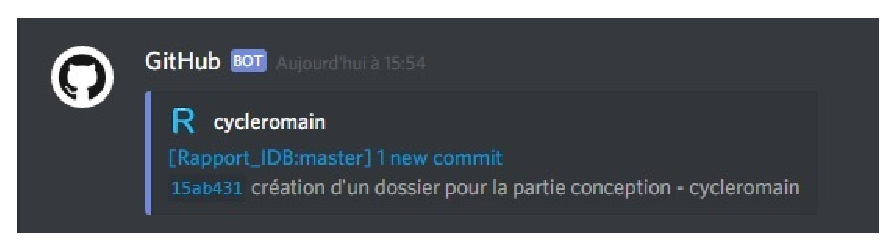
\includegraphics[width=10cm]{./images/activite/bot_discord.eps}
\caption{Message du BOT Discord lié à GitHub}
\label{bot_discord}
\end{figure}



\subsection{Partage de documents}
Tout au long du projet, nous avons produits différents documents qu'il nous a fallu stocker dans un endroit facile d'accès pour tous. Nous avons donc créé un dossier sur un \textbf{Google Drive} (figure \ref{googledrive_logo}) et l'avons partagé aux membres du groupe. Ce Drive nous a permis d'échanger et stocker des diagrammes, des pdfs, des documents texte, des maquettes pour les \glspl{ihm}* ainsi que d'autres fichiers que nous voulions conserver.

\begin{figure}[!h]
\centering

\includegraphics[width=10cm]{./images/activite/googleDriveLogo.eps}
\caption{Logo Google Drive}
\label{googledrive_logo}
\end{figure}





\backmatter

\chapter{Résumé}
\textbf{IDB} est un logiciel gratuit permettant d'utiliser un SGBD* au moyen d'une interface graphique. Son interface est intuitive et permet à un utilisateur, même non informaticien, de manipuler très facilement des tables et les données qu'elles contiennent, mais aussi d'effectuer des requêtes simples (en allant jusqu'aux jointures) sans se soucier du langage SQL*.
\\
Le logiciel est entièrement codé en langage Java (nécessite au minimum JRE* 1.7) et se base sur la bibliothèque JDBC* pour réaliser la communication avec la base de données. Il est entièrement compatible avec les système de gestion de base de données Oracle Database et MySQL.
\bigbreak
Mots clés : base de données, JAVA, JDBC, SQL, interface graphique, Oracle, MySQL, QBE

\bigbreak
\rule{\linewidth}{0.4pt}
\bigbreak

\textbf{IDB} is a free software intended to handle the administration of a database management system with the use of a GUI*. Its use is intuitive and allow non-IT people to manage tables and their data, but also to perform simple queries (even join clause) without having to know SQL*.
\\
This software is written in Java language (requires JRE* 1.7+) and uses the JDBC* tool from Java language to achieve communication with the database management system. It's fully compatible with Oracle Database and MySQL.
\bigbreak
Keywords : database, JAVA, JDBC, SQL, graphical user interface, Oracle, MySQL, QBE


\end{document}
